\PassOptionsToPackage{unicode=true}{hyperref} % options for packages loaded elsewhere
\PassOptionsToPackage{hyphens}{url}
%
\documentclass[]{article}
\usepackage{lmodern}
\usepackage{amssymb,amsmath}
\usepackage{ifxetex,ifluatex}
\usepackage{fixltx2e} % provides \textsubscript
\ifnum 0\ifxetex 1\fi\ifluatex 1\fi=0 % if pdftex
  \usepackage[T1]{fontenc}
  \usepackage[utf8]{inputenc}
  \usepackage{textcomp} % provides euro and other symbols
\else % if luatex or xelatex
  \usepackage{unicode-math}
  \defaultfontfeatures{Ligatures=TeX,Scale=MatchLowercase}
\fi
% use upquote if available, for straight quotes in verbatim environments
\IfFileExists{upquote.sty}{\usepackage{upquote}}{}
% use microtype if available
\IfFileExists{microtype.sty}{%
\usepackage[]{microtype}
\UseMicrotypeSet[protrusion]{basicmath} % disable protrusion for tt fonts
}{}
\IfFileExists{parskip.sty}{%
\usepackage{parskip}
}{% else
\setlength{\parindent}{0pt}
\setlength{\parskip}{6pt plus 2pt minus 1pt}
}
\usepackage{hyperref}
\hypersetup{
            pdftitle={Converser à l'ère de l'autocomplétion},
            pdfauthor={Mathilde Buenerd, Tuteur: Nicolas Nova},
            pdfborder={0 0 0},
            breaklinks=true}
\urlstyle{same}  % don't use monospace font for urls
\usepackage{graphicx,grffile}
\makeatletter
\def\maxwidth{\ifdim\Gin@nat@width>\linewidth\linewidth\else\Gin@nat@width\fi}
\def\maxheight{\ifdim\Gin@nat@height>\textheight\textheight\else\Gin@nat@height\fi}
\makeatother
% Scale images if necessary, so that they will not overflow the page
% margins by default, and it is still possible to overwrite the defaults
% using explicit options in \includegraphics[width, height, ...]{}
\setkeys{Gin}{width=\maxwidth,height=\maxheight,keepaspectratio}
\usepackage[normalem]{ulem}
% avoid problems with \sout in headers with hyperref:
\pdfstringdefDisableCommands{\renewcommand{\sout}{}}
\setlength{\emergencystretch}{3em}  % prevent overfull lines
\providecommand{\tightlist}{%
  \setlength{\itemsep}{0pt}\setlength{\parskip}{0pt}}
\setcounter{secnumdepth}{0}
% Redefines (sub)paragraphs to behave more like sections
\ifx\paragraph\undefined\else
\let\oldparagraph\paragraph
\renewcommand{\paragraph}[1]{\oldparagraph{#1}\mbox{}}
\fi
\ifx\subparagraph\undefined\else
\let\oldsubparagraph\subparagraph
\renewcommand{\subparagraph}[1]{\oldsubparagraph{#1}\mbox{}}
\fi

% set default figure placement to htbp
\makeatletter
\def\fps@figure{htbp}
\makeatother


\title{Converser à l'ère de l'autocomplétion}
\author{Mathilde Buenerd, Tuteur: Nicolas Nova}
\date{Janvier 2018}

\begin{document}
\maketitle

\newpage

\hypertarget{converser-uxe0-luxe8re-de-lautocompluxe9tion}{%
\section{Converser à l'ère de
l'autocomplétion}\label{converser-uxe0-luxe8re-de-lautocompluxe9tion}}

\emph{Relecture critique des caractéristiques que l'on attribue au
design d'interaction (\emph{design invisible}, \emph{technologie calme},
\emph{utilisabilité}), dans le cadre des systèmes d'aide à l'écriture et
à la conversation, et particulièrement de l'autocomplétion}

Mathilde Buenerd

Tuteur : Nicolas Nova

Haute Ecole d'Art et de Design (HEAD), Genève Master HES-SO, Media
design

imprimé en février 2017

\newpage

\hypertarget{remerciements}{%
\subsection{Remerciements}\label{remerciements}}

\newpage

\hypertarget{notes}{%
\paragraph{Notes}\label{notes}}

Les mots en italique entre {[}\emph{crochets}{]} sont utilisés pour
clarifier la référence à des mots anglais pour lesquels un équivalent
français n'est pas évident.

Tous les liens hypertextes des articles cités sont dans la
bibliographie.

Le texte est disponible en ligne à l'adresse\\
mathilde.buenerd.fr/converser-a-l-ere-de-l-autocompletion

\newpage

\hypertarget{sommaire}{%
\subsection{Sommaire}\label{sommaire}}

\newpage

\hypertarget{introduction}{%
\subsection{Introduction}\label{introduction}}

\emph{Regime of computation} (Hayles 2005), \emph{Age of the algorithm}
(Finn 2017), ou encore \emph{``logicialisation''} de la société (Citton
2015), autant de termes pour désigner un même phénomène : la place
grandissante du logiciel {[}\emph{software}{]} dans la société, à une
échelle importante et dans des domaines variés : travail, finance,
relations sociales etc. Une ère dominée par la figure de l'algorithme
comme structure ontologique de compréhension de l'univers (Finn 2017,
21).

Une incarnation du logiciel dans la vie quotidenne concerne la
multiplication des assistants personnels ou de ce qu'on pourrait nommer
des \emph{machines sociales} (Hendler and Mulvehill (auth.) 2016, 10),
au sens d'ordinateurs qui ont la capacité d'interagir dans un espace
social traditionnellement réservé aux humains. C'est le cas des
applications de messagerie (email) ou de messagerie instantanée
(Messenger, Whatsapp et autres) ou encore des assistants personnels
(Siri, Alexa\ldots{}). Plus que de simples intermédaires, ces services
impliquent de nouvelles manières d'écrire, d'échanger, et au final, de
converser. Ces nouvelles manières de s'exprimer sont permises entre
autres par des fonctionnalités telles que l'autocomplétion.

L'autocomplétion désigne la fonctionnalité informatique consistant à
compléter les mots qu'un usager a commencé à saisir. C'est une
fonctionnalité majeure sur le web et dans les applications de
conversation à distance. Elle devient une caractéristique incontournable
dans le design de l'expérience utilisateur, en témoignent la
multiplication de widgets comme
\href{http://jqueryui.com/}{\emph{autocomplete}} du populaire jQueryUI
(collection d'outils à destination des développeurs pour faciliter la
création de sites internet). Synonyme de \emph{complètement},
\emph{complètement automatique} ou encore \emph{saisie intuitive} ou
\emph{saisie prédicitive}, le terme d'\emph{autocomplétion} a été choisi
ici pour sa proximité avec le terme anglais \emph{autocomplete},
largement employé dans le monde de la programmation informatique.

Derrière son allure insignifiante, l'autocomplétion est une
fonctionnalité que l'on utilise quotidiennement et qui touche un aspect
intime de notre vie : les correspondances que l'on a avec nos proches
via nos appareils électroniques. En même temps, c'est aussi un exemple
de technologie qu'on ne remarque pas. On rit parfois d'une suggestion
inappropriée, on s'étonne (ou s'effraie) de la justesse d'une
proposition qu'on avait sur le bout de la langue. Mais notre
compréhension du système est généralement limitée, c'est une
fonctionnalité un peu discrète (ou totalement invisible) et un peu
futile (ou peu magique).

On peut être tenté de penser que l'autocomplétion est avant tout un
problème technique, un problème d'ingéniérie : comment prédire les mots
que l'utilisateur va écrire ? L'enjeu serait avant tout d'améliorer la
précision des prédictions, et c'est probablement pourquoi toutes les
interfaces (Whatsapp, Messenger, Allo\ldots{}) se ressemblent fortement
: l'esthétique des interfaces est interchangeable; et l'expérience
utilisateur est standardisée. On pourrait également penser que l'enjeu,
c'est la compréhension du langage naturel par les machines. En 1950, en
définissant un ordinateur intelligent comme un ordinateur capable
d'\emph{imiter} le langage humain de manière suffisement convaincante,
le test de Turing donne à la compréhension du langage une place
prépondérante dans le champ d'étude qu'on appelera bientôt
\emph{intelligence artificielle} (Turing 1950). Quelques années plus
tard, Joseph Weizenbaum épate le monde scientifique avec ELIZA, un
programme informatique qui simule un psychothérapeute avec lequel un
interlocuteur humain peut converser via un clavier (Weizenbaum 1981,
121--33).\\
À l'origine, les chercheurs supposaient que cette compréhension du
langage serait possible à condition de pouvoir définir précisement le
langage avec des règles. Mais la complexité de décrire l'intégralité des
éléments qui consituent la langue a rapidement suscité de nombreuses
désillusions (Weizenbaum 1981, 5--11), et aujourd'hui encore, nous ne
discutons toujours pas quotidiennement avec des robots. Si ce champ de
recherche est passionant, il ne doit pas éclipser d'autres enjeux qui
sont aujourd'hui négligés, en particulier des enjeux de design
d'expérience et d'interface.

\hypertarget{lautocompluxe9tion-change-notre-maniuxe8re-duxe9changer}{%
\paragraph{L'autocomplétion change notre manière
d'échanger}\label{lautocompluxe9tion-change-notre-maniuxe8re-duxe9changer}}

Que ce soit de manière fortuite ou délibérée, les outils modèlent notre
manière de parler. Un aspect de la tranformation du langage par les
algorithmes est ce que Tarleton Gillespie appelle la ``négociation
tacite'' {[}\emph{tacit negociation}{]} (Gillespie (ed.), Boczkowski
(ed.), and Foot (ed.) 2014, 184), c'est-à-dire qu'on adapte -
délibérément ou non - son comportement pour tirer parti de l'algorithme.
On ajuste son phrasé pour se rendre plus intelligible par Siri, on
choisit conscieusement des hashtags pour que son contenu soit affiché
dans le fil d'actualité, on rédige son site web avec des termes ``search
engine-friendly.''\footnote{L'optimisation délibérée des contenus pour
  les rendre plus facilement indexables par un algorithme n'est que
  l'aspect le plus visible de cette négociation tacite. Parmi d'autres
  aspects Gillepsie cite le recours à des hashtags populaires pour se
  faire remarquer, ou encore les utilisateurs que P2P qui font
  délibéremment des fautes de frappes pour ``cacher'' un contenu
  illégal.}\\
Parce que l'autocomplétion impacte notre manière de parler et
d'échanger, et que celle-ci est un élément clé dans la gestion de nos
relations sociales, le design de tels systèmes doit être
consciencieusement réfléchi.

\hypertarget{pruxe9sentation-du-muxe9moire}{%
\subsubsection{Présentation du
mémoire}\label{pruxe9sentation-du-muxe9moire}}

Le design de tels systèmes, c'est-à-dire les décisions relatives à leur
aspect et à l'interaction avec l'usager, se place dans le champ du
design d'expérience et d'interface {[}\emph{user experience}, \emph{user
interface}{]}. Mais est-ce que les concepts sur lesquels s'appuit le
design de l'expérience utilisateur sont adaptés au design des systèmes
d'autocomplétion ? Le présupposé est que non, c'est pourquoi, pour
analyser les enjeux de l'autocomplétion, ce mémoire vise à faire une
relecture critique de trois notions relatives au design d'interaction :
le design invisible {[}\emph{invisible design}{]}, la technologie calme
{[}\emph{calm technology}{]} et la notion d'utilisabilité.

En premier lieu, il s'agira d'expliquer pourquoi l'évolution du
fonctionnement technique des systèmes d'autocomplétion, notamment grâce
aux algorithmes de \emph{machine learning}, nécessitent de repenser la
manière dont on les conçoit (partie 1). Ensuite, trois idées seront
développées : celles d'un design visible, perturbant et qui pousse à
l'inventivité (parties 2 à 4). Au centre de ces thématiques se trouvent
deux grandes questions : comment le design d'interface peut rendre
intelligible comment un système fonctionne ? Comment penser des formes
de technologies qui ne sont pas juste auxiliaires, mais provocatrices,
excitantes ? La dernière partie sera dédiée à un questionnement plus
large sur la collaboration humain-machine, et à la définition de la
notion de \emph{technologie chili} comme alternative aux tendances
évoquées dans les chapitres précédents (partie 5). Enfin, une annexe
présentera des exemples d'application des principes évoqués au cours du
mémoire, dans le cadre d'une application de messagerie fictionnelle.

Ce mémoire n'est pas une contestation unilatérale des principes ou des
mouvements évoqués, mais plutôt une invitation à sortir de la rhétorique
de ``l'invisibilité'' ou de ``l'intuitivité'' qu'on attribue au design
d'interaction. Ce changement de perspective est là pour réimaginer les
interactions humain-machine dans une optique où l'humour, la provocation
et l'excitation sont au centre des préoccupations.

\newpage

\hypertarget{du-systuxe8me-dautocompluxe9tion-au-systuxe8me-de-recommandation}{%
\subsection{Du système d'autocomplétion au système de
recommandation}\label{du-systuxe8me-dautocompluxe9tion-au-systuxe8me-de-recommandation}}

\hypertarget{dune-aide-uxe0-la-saisie-vers-une-aide-uxe0-luxe9criture}{%
\subsubsection{D'une aide à la saisie vers une aide à
l'écriture}\label{dune-aide-uxe0-la-saisie-vers-une-aide-uxe0-luxe9criture}}

Dans le champ de la téléphonie mobile, l'autocomplétion est présente
depuis plusieurs années en tant qu'aide à la saisie. A la fin des années
90, la majorité des terminaux mobiles possèdent un clavier à 12
chiffres, proche de celui des cadrans téléphoniques. Il est conçu avant
tout pour la saisie de numéros de téléphone et pas pour celle de textos.
Pour pouvoir y saisir du texte, chaque touche possède plusieurs lettres
associées (par exemple le `2' sert aussi à saisir les lettres `a', `b'
et `c'), ce qui implique un problème de désambiguïsation
{[}\emph{disambiguation}{]} lors de la saisie : comment savoir si
l'usager a voulu taper un `a', un `b' ou un `c' ? Les développeurs ont
recours à des méthodes d'entrée pragmatiques, comme le
\emph{mutli-press} (presser une fois pour `a', deux fois pour `b', trois
fois pour `c') ou le \emph{two-keys} (presser `abc' puis `1' pour `a',
`abc' puis `2' pour `b', etc.)\footnote{Pour un historique plus détaillé
  des différentes méthodes de disambiguation, voir (Silfverberg,
  MacKenzie, and Korhonen 2000).}. De manière plus originale, des
systèmes comme le T9\footnote{\emph{``text on 9 keys''}, basé sur les
  travaux de Scott Minneman et développé par Tegic Communications Inc.~à
  la fin des années 90. On peut aussi citer l'iTap (Motorola) ou la
  technologie LetterWise qui ont une approche assez similaire.} adoptent
une approche linguistique basée sur un dictionnaire comportant tous les
mots de la langue (Grover, King, and Kushler 1998). Bien que plusieurs
lettres soient associées à une même touche, une séquence de touches ne
pourra produire qu'un petit nombre de mots\footnote{On estime à à peine
  5\% la probabilité d'erreur de prédiction grâce à cette approche
  linguistique (Silfverberg, MacKenzie, and Korhonen 2000).}. En
combinant cela au fait que les mots ont des fréquences différentes (`tu'
est beaucoup plus fréquent que `accordéon'), on obtient un système
capable de \emph{prédire} quel mot a le plus de chance d'être écrit.
C'est d'ailleurs le terme de ``texte prédictif'' {[}\emph{predictive
text}{]} qui est adopté pour désigner cette technologie de complétion.

Bien que visant à résoudre le problème d'ambiguïté de la saisie, le T9
introduit une méthode de saisie qui comporte des similarités avec les
systèmes d'autocomplétion actuels, c'est-à-dire parier sur un mot en se
basant sur des données (un dictionnaire) et des probabilités (les
fréquences).

\hypertarget{lautocompluxe9tion-aujourdhui}{%
\subsubsection{L'autocomplétion
aujourd'hui}\label{lautocompluxe9tion-aujourdhui}}

\begin{figure}
\centering
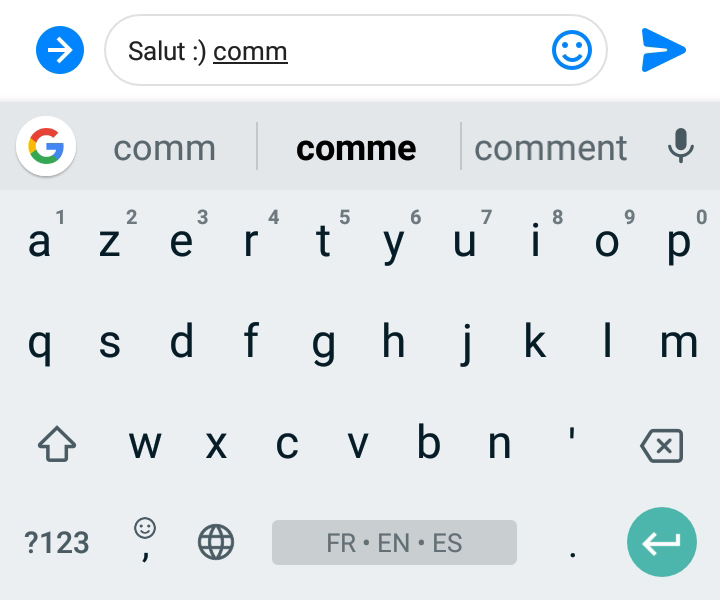
\includegraphics{./tex2pdf.9048/9a827d1ae408fae7a806fb6dc0ac9905e541305a.jpg}
\caption{Type 1 : Le système cherche à trouver la fin du mot qui
commence par ``comm''}
\end{figure}

\begin{figure}
\centering
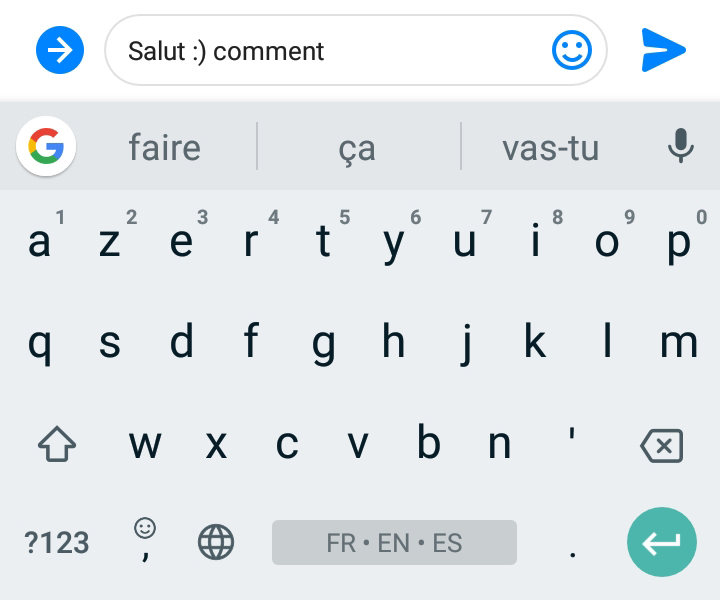
\includegraphics{./tex2pdf.9048/7e321247293e59f1206e6e8fa909f249ef6be4d8.jpg}
\caption{Type 2 : Le système cherche à trouver le mot qui suit le mot
``comment''}
\end{figure}

Aujourd'hui, on peut distinguer deux types d'autocomplétion. La première
est celle qui vient compléter les mots que l'on a commencé à saisir.
C'est la descendante directe de systèmes comme le T9 et des correcteurs
orthographiques. Elle est plutôt une aide à la saisie, corrige les
fautes d'orthographe et augmente la vitesse d'écriture.\\
La seconde est celle qui vient suggérer des mots ou des phrases
complètes, en se basant sur le début de notre phrase ou de celle de
notre interlocuteur. Elle est plus proche d'une aide à l'écriture, dans
la mesure où elle est plus envahissante. Ce type d'autocomplétion tente
de prédire ce que l'on veut dire en se basant sur les mots déjà écrits,
et sur les fréquences d'association des mots entre eux (par exemple une
phrase qui commence par ``Merci'' a plus de chances d'être suivie de
``beaucoup'' que de ``accordéon''). Ces fréquences sont calculées grâce
à une approche statistique de la langue qui consiste à analyser des
ensembles de milliers de textes appelés \emph{corpus}.

Recourir à des statistiques et des probabilités pour prédire ou
anticiper les actions de quelqu'un, c'est l'idée au centre d'un champ
d'étude de l'intelligence artificielle particulièrement en vogue, le
\emph{machine learning}\footnote{En 2017, ``machine learning'' et ``deep
  learning'' (une méthode spécifique d'application du machine learning)
  étaient tout en haut du ``pic des attentes exagérées'' {[}\emph{peak
  of inflated expectations}{]} du
  \href{https://blogs.gartner.com/smarterwithgartner/files/2017/08/Emerging-Technology-Hype-Cycle-for-2017_Infographic_R6A.jpg}{Gartner
  Hype Cycle}.}, qu'on peut traduire en français par \emph{apprentissage
automatique}. Ces algorithmes font fonctionner les assistants personnels
comme Siri et produisent les recommandations personnalisées de Spotify
ou d'Amazon. Ces programmes cherchent à prédire un comportement futur en
se basant sur une analyse statistique des comportements passés. Ils
apprenent du comportement de l'usager, et évoluent en fonction de ses
habitudes. Le corollaire d'une telle technique consiste en une
personnalisation grandissante de l'expérience utilisateur : le programme
``s'adapte'' à chaque individu.

La place centrale qu'a pris la prédiction dans les systèmes
d'autocomplétion fait qu'on peut les définir comme des \emph{systèmes de
recommandation pour l'écriture}. C'est-à-dire, des systèmes qui
cherchent à prédire la préférence d'une personne pour un mot, une
phrase, un emoji ou une idée.

\hypertarget{ruxe9pondre-sans-taper-dans-son-propre-style}{%
\subparagraph{``Répondre sans taper, dans son propre
style''}\label{ruxe9pondre-sans-taper-dans-son-propre-style}}

\begin{figure}
\centering
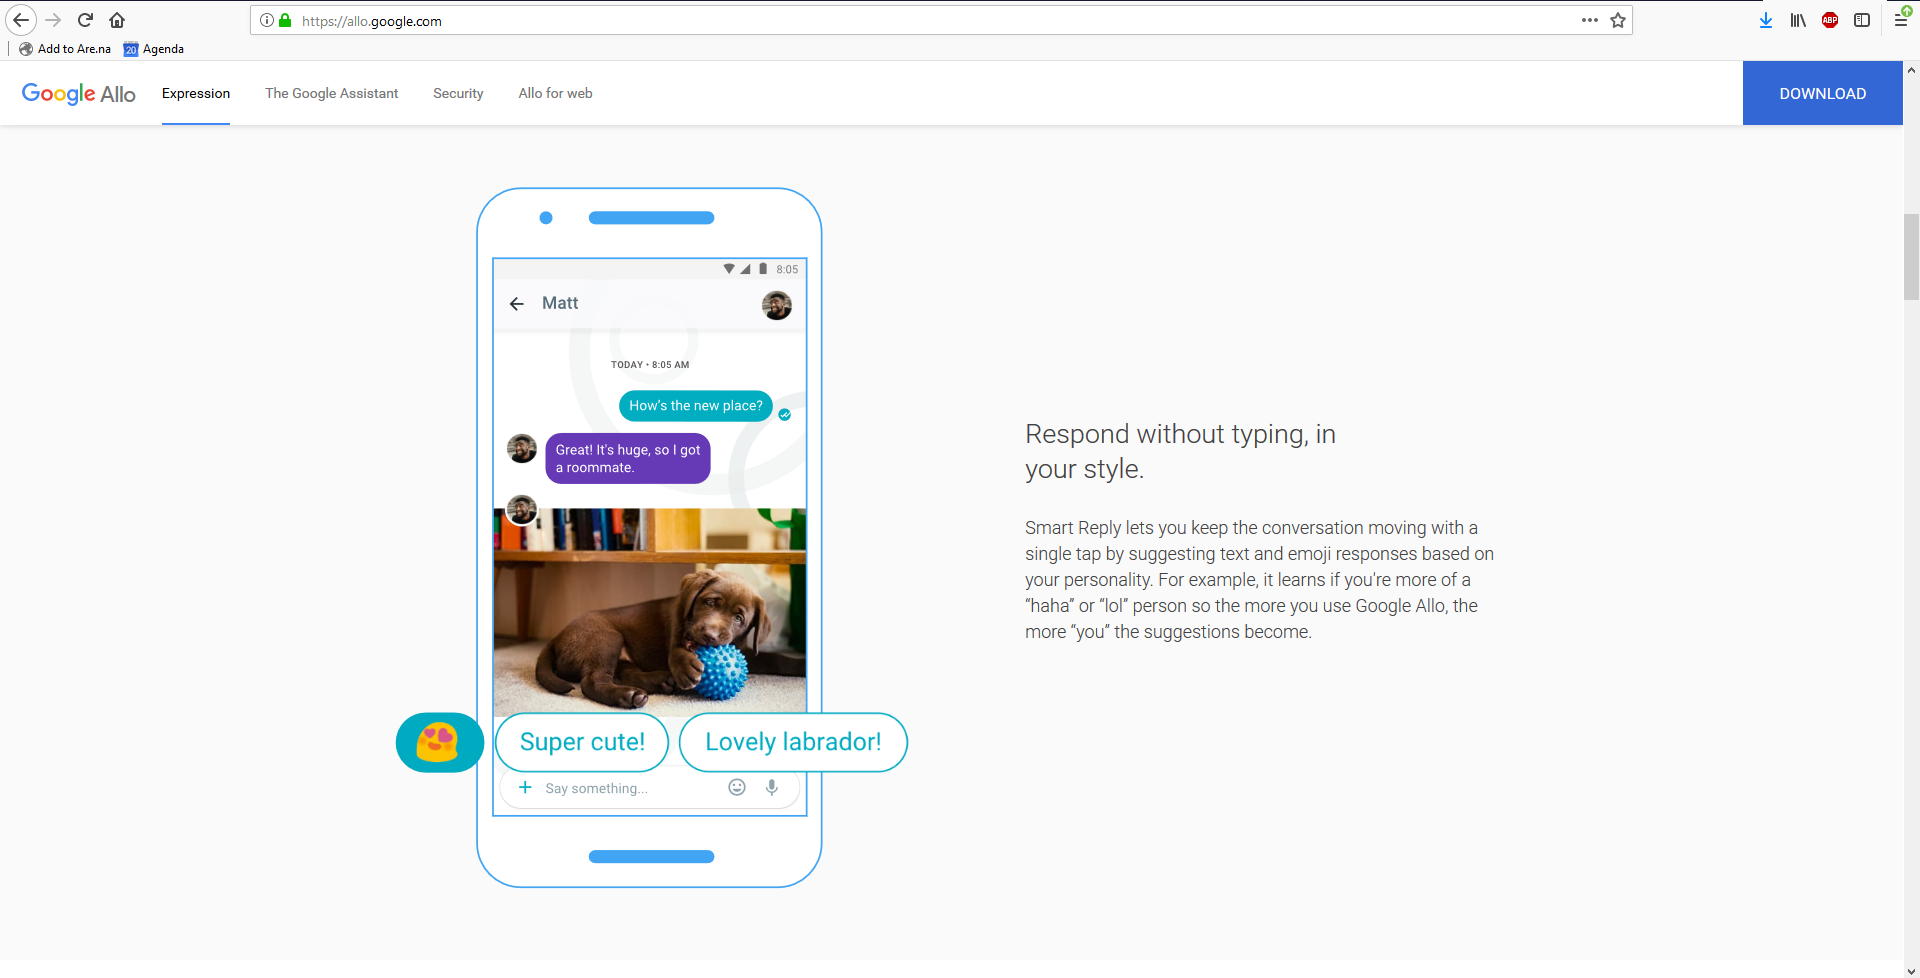
\includegraphics{./tex2pdf.9048/4781b0ca038539d65002c9935802db7dd11ab3ba.png}
\caption{Google Allo : ``Répondre sans taper, dans son propre style''}
\end{figure}

Un exemple-type de système de recommandation pour l'écriture, est
l'application de messagerie instantanée développée par Google, Google
Allo. Cette application de messagerie ``intelligente'' suggère des
réponses-type en fonction des habitudes d'écriture. Elle retient par
exemple si vous êtes une personne plutôt ``dac'' ou ``ok'', et intègre
des suggestions à l'intérieur même des conversations grâce à un
assistant semblable à Siri. Google Allo n'est pas la seule application à
aller jusqu'à suggérer des mots ou des réponses préétablies. La
messagerie en ligne Gmail et Facebook les utilisent aussi.

\begin{figure}
\centering
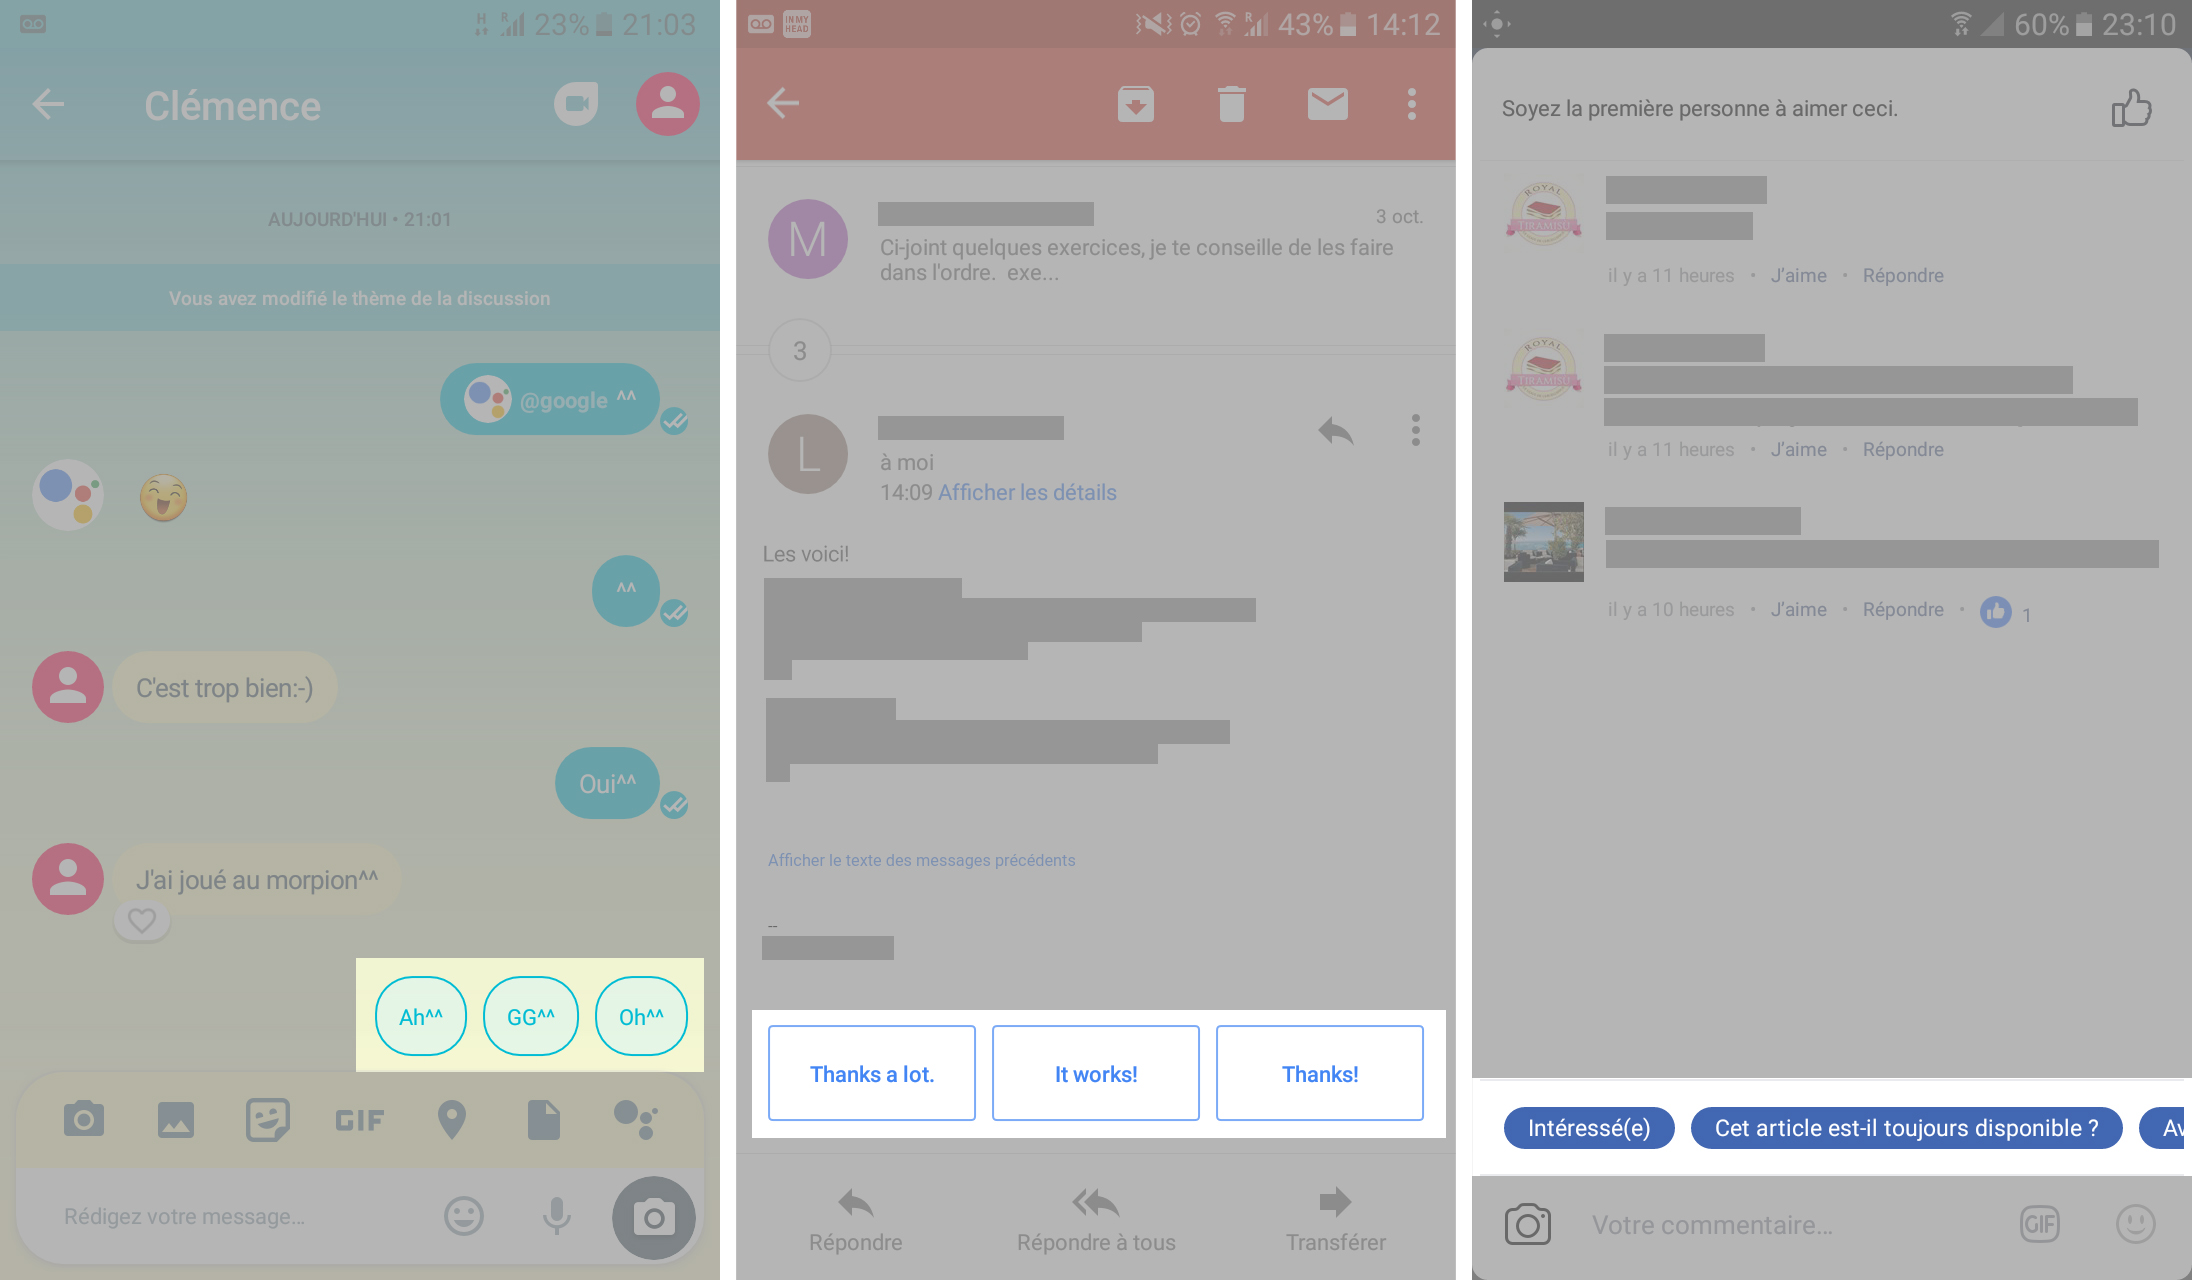
\includegraphics{./tex2pdf.9048/f533f83856416ad4ef1cb780738ceed366251b8c.jpg}
\caption{Réponses automatiques sur Google Allo, Gmail et Facebook}
\end{figure}

Dans le cas de ces deux dernières applications, les suggestions sont
basées sur une analyse statistique des réponses écrites non pas par
l'usager lui-même mais par les usagers en général. S'il est difficile de
savoir exactement comment ces réponses sont produites, il est probable
qu'elles ne résultent pas d'un algorithme autonome, car elles ne sont
présentes que dans le cas de situations standardisées, par exemple
``Merci'' ou ``Bien reçu''. Néanmoins, on peut voir dans ces nouvelles
fonctionnalités une porte ouverte vers l'usage d'algorithmes de machine
learning pour faire de la recommandation conversationnelle.

\hypertarget{fonctionnement-dun-systuxe8me-de-recommandation}{%
\subsubsection{Fonctionnement d'un système de
recommandation}\label{fonctionnement-dun-systuxe8me-de-recommandation}}

Comprendre les grands principes de fonctionnement d'un système de
recommandation permet de mieux apprécier leurs spécificités, leurs
contraintes et leurs avantages, et ainsi de pouvoir les concevoir d'un
point de vue de design d'expérience. Sans entrer le détail, on peut
distinguer deux grandes catégories de système de recommandation : ceux
basés sur le contenu et ceux dit ``collaboratifs.''\footnote{En
  pratique, ces systèmes sont généralement hybrides, ils mélangent ces
  deux approches.} Le schéma ci-dessous donner un aperçu de leurs
caratéristiques.

\begin{figure}
\centering
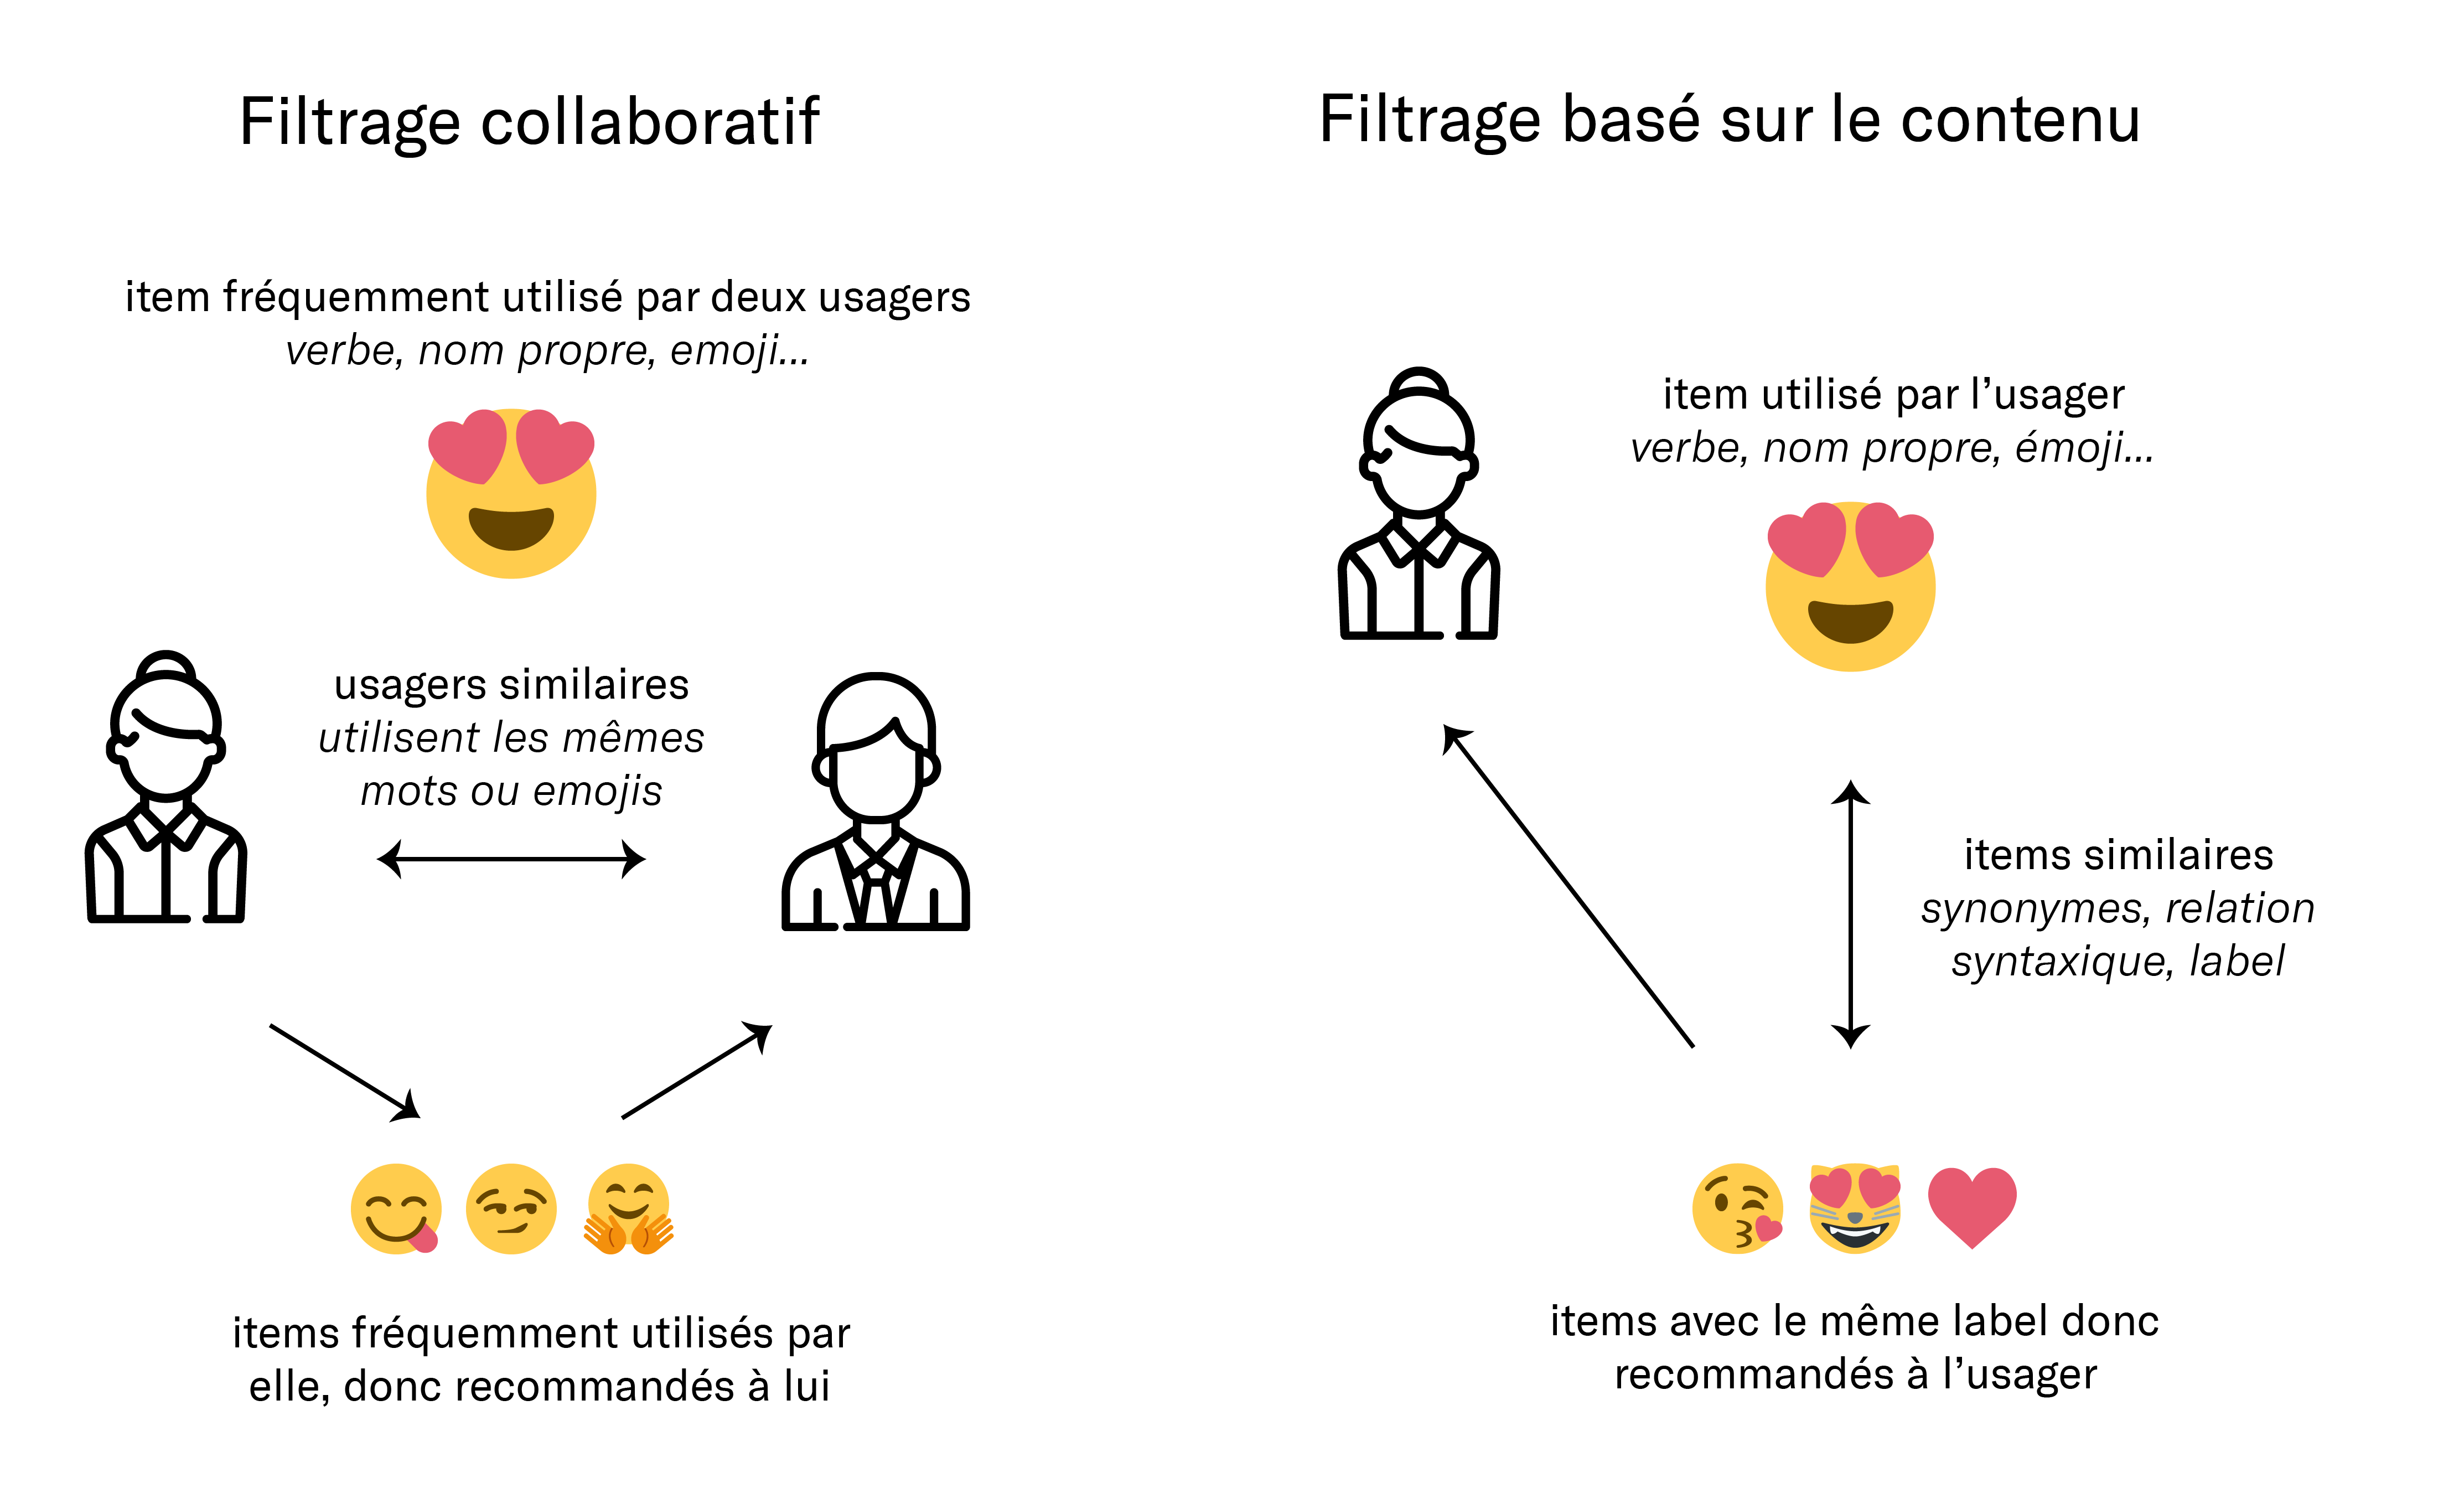
\includegraphics{./tex2pdf.9048/734eb3977aec2f5d5847ce3bde5b018c6fe2c10c.png}
\caption{Deux types de systèmes de recommandation}
\end{figure}

Dans le cas de l'autocomplétion, on pourrait par exemple différencier un
système basé sur le contenu, qui recommenderait des mots liés par une
relation de sens ou de syntaxe (par exemple un synonyme connu grâce à un
dictionnaire) et des mots liés par un comportement collectif (par
exemple des mots souvent associés par l'ensemble des usagers).

\hypertarget{design-dun-systuxe8me-dun-systuxe8me-de-recommandation}{%
\subsubsection{Design d'un système d'un système de
recommandation}\label{design-dun-systuxe8me-dun-systuxe8me-de-recommandation}}

Si l'on commence à désigner les systèmes d'autocomplétion comme des
systèmes de recommandation pour l'écriture, alors on peut se poser la
question de comment les problèmes qui se posent actuellement aux
systèmes de recommandation peuvent les impacter. Sans en faire une liste
exhaustive, on peut citer trois grandes questions : celle de la
régularisation de la langue, du déterminisme qu'implique un système qui
s'autoalimente et la gestion délicate des données personnelles.

\hypertarget{la-ruxe9gularisation-de-la-langue}{%
\subparagraph{La régularisation de la
langue}\label{la-ruxe9gularisation-de-la-langue}}

On adapte son langage quand on utilise des systèmes électroniques. Mais
les apps de messagerie modèlent notre manière de parler en retour. Se
basant sur une approche statistique de la langue, l'autocomplétion peut
réduire sa richesse en poussant les usagers à employer les mots qui sont
statistiquement les plus fréquents. Sans être en mesure de prouver une
transformation générale de la langue par l'autocomplétion, on peut
émettre l'hypothèse d'une tendance générale vers une expression
linguistique plus régulière et moins idiomatique. Une expression qui
défavoriserait des aspects comme les fautes d'orthographe, le registre
de langue familier, ou les mots régionaux. C'est que Kaplan appelle le
``capitalisme linguistique'' (Kaplan 2014) : Google a un intérêt
financier à ce que les requêtes des utilisateurs soient les plus
compréhensibles. Sous cet angle, l'objectif et l'effet des outils de
correction et d'autocomplétion est d'homogénéiser la langue.\footnote{Voir
  aussi l'extension de la métaphore financière par Pip Thornton, qui
  parle de la possible création d'un ``langage subprime'' (Thornton
  2017).}\\
Dans ce cas, la diversification de la langue par l'autocomplétion peut
être vue comme un contrepied à cette uniformisation. Par exemple en ne
sanctionnant pas systématiquement les fautes d'orthographe, ou en
proposant des mots insolites.

\hypertarget{la-bulle-de-filtres}{%
\subparagraph{La ``bulle de filtres''}\label{la-bulle-de-filtres}}

\begin{quote}
But when algorithms cross the threshold from prediction to
determination, from modeling to building cultural structures, we find
ourselves revising reality to accommodate their discrepancies. (Finn
2017, 50)
\end{quote}

Plus on se fie à des recommandations, plus elles nous façonnent. Il y a
toujours le risque que les algorithmes quittent le monde de la
prédiction pour entrer dans celui de la détermination, en créant un
système qui s'autoalimente. Le militant internet Eli Pariser alerte
contre le risque que les recommandations créent ce qu'il appelle une
``bulle de filtre'' {[}\emph{filter bubble}{]} (Pariser 2011). Selon
lui, la personnalisation du web, c'est-à-dire l'emploi de l'historique
de recherche et des données personnelles des usagers pour leur faire des
suggestions, reviendrait à confiner chacun dans sa propre bulle
culturelle et idéologique.\\
Mais on peut voir dans l'autocomplétion une opportunité pour justement
élargir cette bulle culturelle. Si l'on imagine par exemple suggérer des
mots désuets à des jeunes, ou bien des mots issus de l'argot des jeunes
à des personnes âgées.

\hypertarget{la-duxe9licate-gestion-des-donnuxe9es-personnelles}{%
\subparagraph{La délicate gestion des données
personnelles}\label{la-duxe9licate-gestion-des-donnuxe9es-personnelles}}

Le revers de la personnalisation, c'est la collecte massive de données
personnelles. Ces données sont récupérées, stockées, analysées. Elles
sont utilisées pour prendre des décisions qui dépassent la réalité
qu'elles nous laissent entrevoir, et parfois avec des conséquences
dramatiques\footnote{Virginia Eubanks dénonce des systèmes automatisés
  aux Etats-Unis ayant pour tâche de répartir l'aide sociale ou évaluer
  un risque d'être victime d'abus sexuels.} ({\textbf{???}}). La
question de la protection de la vie privée est donc centrale. Il faut
garder du recul sur les informations perçue au travers de les profils et
de les comportements, et garder à l'esprit qu'on ne peut pas
rationnaliser la personnalité d'une personne aux données collectées sur
elle. Donner aux gens accès aux données collectées sur eux, et la
capacité de les modifier est donc essentiel.

\hypertarget{vers-de-nouvelles-maniuxe8res-de-designer}{%
\paragraph{Vers de nouvelles manières de
designer}\label{vers-de-nouvelles-maniuxe8res-de-designer}}

Et si l'évolution technologique était telle qu'elle nécessite de penser
différemment la manière dont on conçoit l'expérience des systèmes basés
sur des algorithmes de machine learning ? Si les enjeux centraux n'était
pas tant l'intuitivité ou la facilité d'usage, mais la capacité à
permettre la découverte ou à dépasser ses limites ?\footnote{Pour une
  analyse plus détaillée des liens entre design d'expérience et machine
  learning, voir (Girardin 2016).}

Alors que les possibilités offertes par ces nouveaux algorithmes sont
collossales, on constate que toutes les applications de messagerie se
ressemblent : elle semblent être des variations d'une même application.
Les causes de ce problème sont inévitablement multiples : complexité des
systèmes, problèmes liés à l'interdisciplinarité. Néanmoins, plusieurs
hypothèses issues de l'histoire du design peuvent se réveler
problématiques : le travail de designer se résumerait à la résolution
d'un problème, la technologie ne devrait pas empiéter sur la vie
``réelle'', le bon design est celui qui ne se verrait pas.

Les trois prochains chapitres sont une relecture de ces trois
caractéristiques.

\newpage

\hypertarget{utilisabilituxe9-inventivituxe9}{%
\subsection{\texorpdfstring{\sout{utilisabilité} =\textgreater{}
inventivité}{utilisabilité =\textgreater{} inventivité}}\label{utilisabilituxe9-inventivituxe9}}

L'\emph{utilisabilité} peut se définir par la capacité d'un objet à être
utilisé de manière efficace (atteindre le but prévu), efficiente
(atteindre ce but avec un effort minimal) et générer une satisfaction de
l'utilisateur (être agréable à utiliser)\footnote{Selon la norme ISO
  9241-11. Voir sur Wikipédia
  https://fr.wikipedia.org/wiki/Utilisabilité}.

C'est un concept central dans l'histoire du design : un bon objet est
celui qui résoud un problème et la qualité d'un design se mesurerait à
la l'efficacité avec laquelle il atteint ce but.

Nous verrons d'abord pourquoi il faut se méfier de vouloir exploiter
naïvement la technologie comme une réponse à des problèmes complexes,
puis pourquoi cette quête de l'efficacité n'est pas pertinente dans le
champ de la communication interpersonnelle.

\newpage

\hypertarget{des-expuxe9riences-pleines-de-bonnes-intentions-des-expuxe9riences-critiques}{%
\subsubsection{\textasciitilde{}\textasciitilde{}Des expériences pleines
de bonnes intentions \textasciitilde{}\textasciitilde{} / Des
expériences
critiques}\label{des-expuxe9riences-pleines-de-bonnes-intentions-des-expuxe9riences-critiques}}

\hypertarget{la-prison-des-espuxe9rances-homoguxe8nes-12b9}{%
\paragraph[\emph{La prison des espérances
homogènes}]{\texorpdfstring{\emph{La prison des espérances
homogènes}\footnote{(``"Means Well" Technology and the Internet of Good
  Intentions'' 2015)}}{La prison des espérances homogènes}}\label{la-prison-des-espuxe9rances-homoguxe8nes-12b9}}

On voit apparaître dans la multiplicité des objets connectés, de
nombreux produits qui se targuent de vouloir régler des problèmes
sociétaux. Simples gadgets ou appareils complexes, leur point commun est
que leurs auteurs sont pleins de bonnes intentions, ils viennent avec
une sincère volonté de rendre le monde meilleur. Mais être bien
intentionné n'est pas suffisant pour régler des problèmes complexes, et
ces projets finissent souvent par être maladroits, embarassants, voir
dangereux.\footnote{Par exemple
  \href{https://motherboard.vice.com/en_us/article/paqvn7/dont-fuck-anybody-who-wants-to-get-your-consent-uploaded-to-the-blockchain-legalfling-app}{LegalFling},
  une app qui utilise la technologie de la blockchain pour gérer le
  consentement à avoir une relation sexuelle.} Pour illustrer cela, on
peut comparer deux projets qui s'inscrivent dans le même champ d'action
: l'assistance à la conversation.

\begin{figure}
\centering
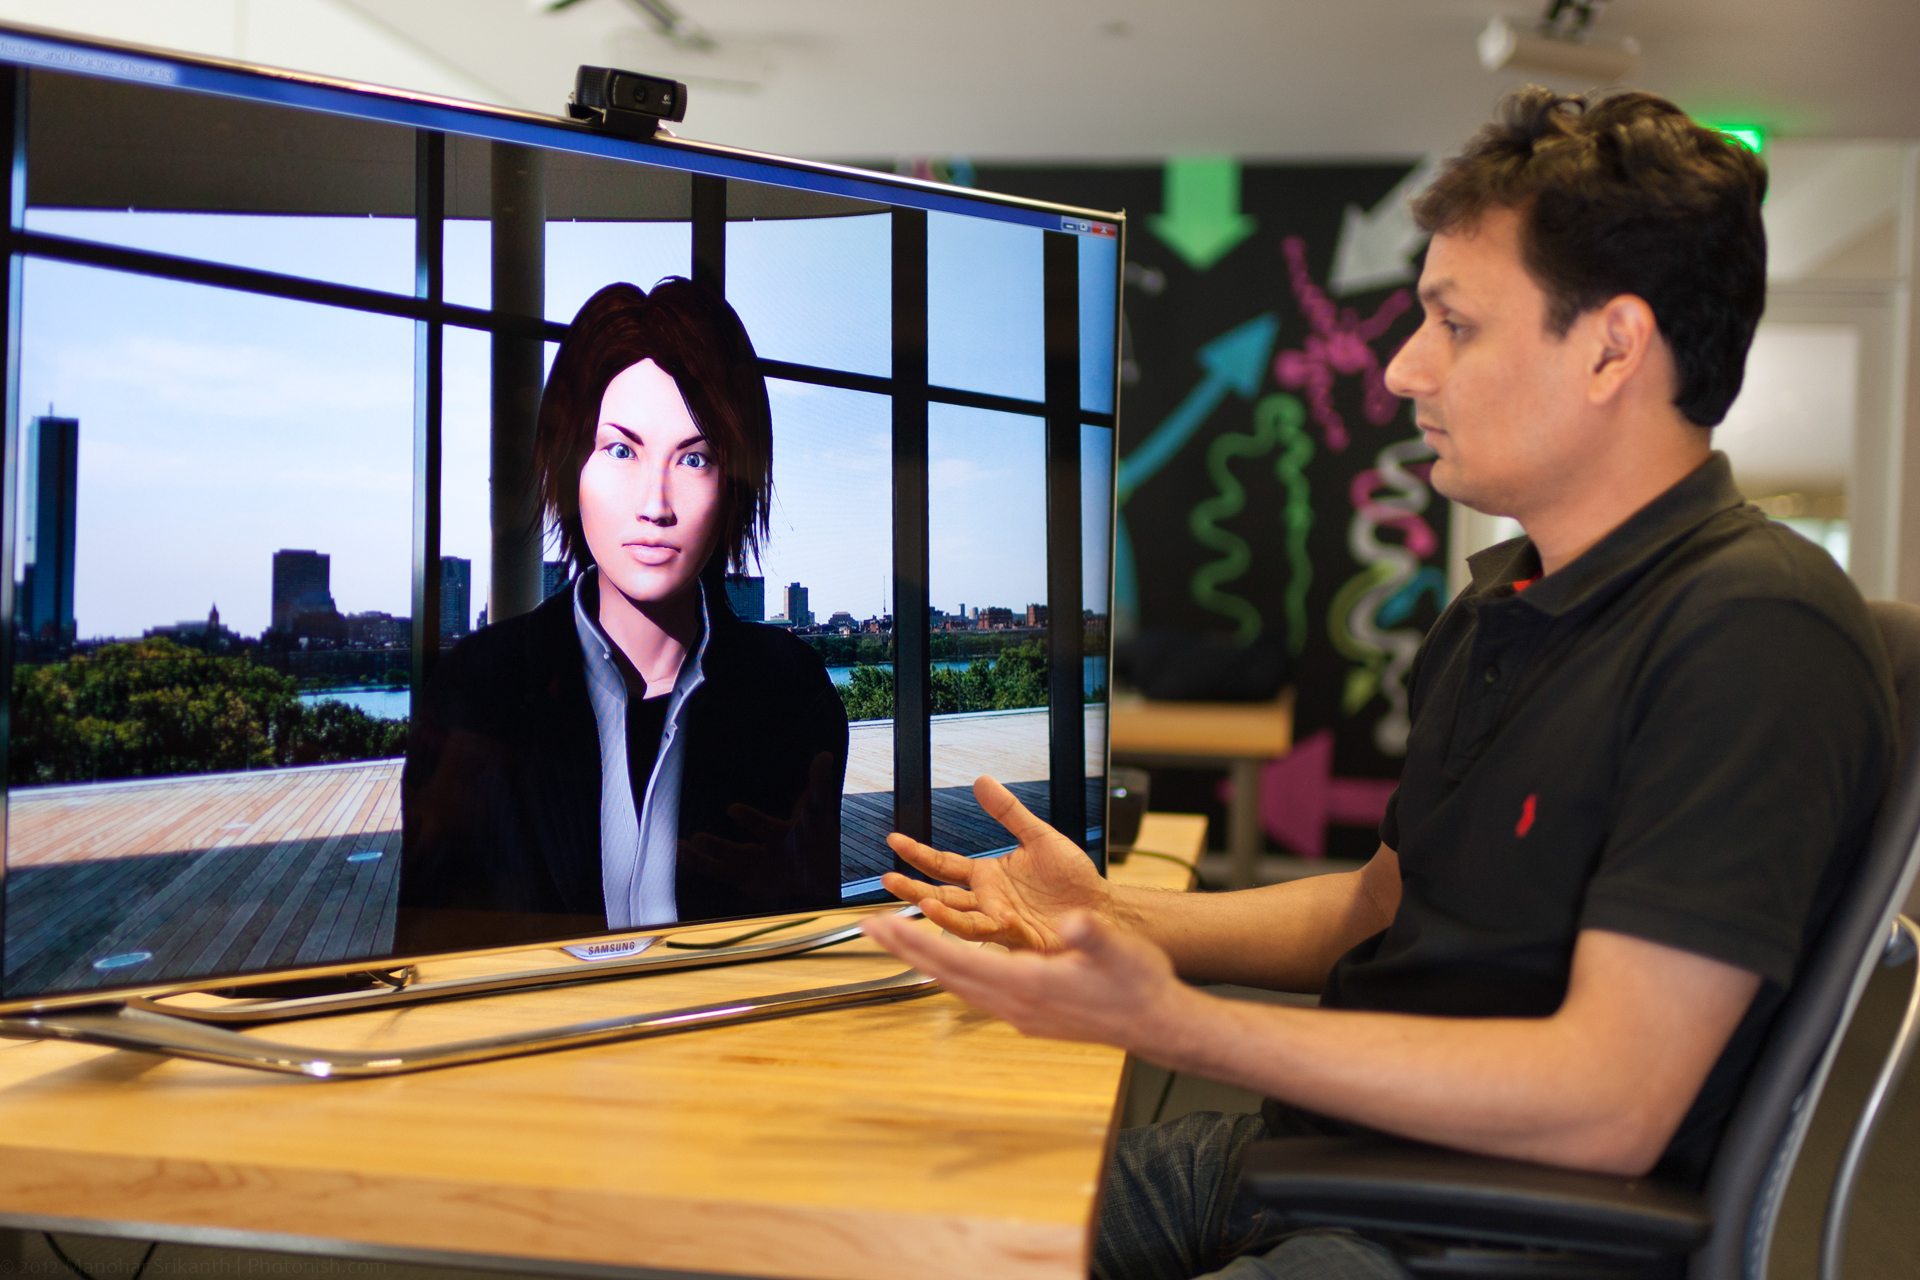
\includegraphics{./tex2pdf.9048/9c6b7392e4842223c2663a48fb2493b3904d4770.jpg}
\caption{MACH}
\end{figure}

Le premier projet vient du laboratoire d'\emph{effective computing}
(littérelement \emph{information efficace}) du MIT Media Lab,
\emph{MACH, My Automated Conversation coacH} (``MACH - My Automated
Conversation coacH,'' n.d.), ``mon coach automatisé pour la
conversation''. C'est un système qui a pour but d'améliorer sa posture
et sa manière de parler lors des conversations en face-à-face.
L'expérience consiste à converser avec un personnage 3D qui répond et
réagit en temps réel. Il peut en outre prendre des initiatives comme
interrompre une personne qui serait trop bavarde. Après la discussion,
le logiciel fournit un bilan détaillé de l'interaction : la fréquence
des sourires, des hochements de tête, des modulations de la voix, la
quantité de ``mots faibles'' (très, bien, en fait\ldots{}), le débit de
parole.

Le logiciel énonce les objectifs à atteindre pour améliorer sa
performance et fournit des graphiques pour comparer les différentes
sessions d'entraînement. Le projet est présenté comme une aide pour
améliorer ses compétences sociales, notamment avec
\href{https://www.youtube.com/watch?v=CHVNOiCT8vA}{des vidéos
avant/après} qui illustrent les réussites du dispositif das le contexte
d'entretiens d'embauche.

Le second projet, \href{http://lauren-mccarthy.com/us}{\emph{us+}}, par
les artistes Lauren McCarthy et Kyle McDonald, est une application de
vidéoconférence Google Hangouts. Son objectif affiché est d'optimiser la
conversation en analysant les expressions faciales et le contenu
linguistique grâce à des algorithmes pouvant extraire des tendances
comportementales comme la positivité, l'agressivité ou la féminité.
Cette analyse est retransmise en direct à l'utilisateur avec des
graphiques en barres. En plus de cette visualisation, l'application
affiche des notifications qui donnent des conseils comme ``Tu parles
beaucoup trop'', et peut effectuer des actions concrètes comme couper le
son.
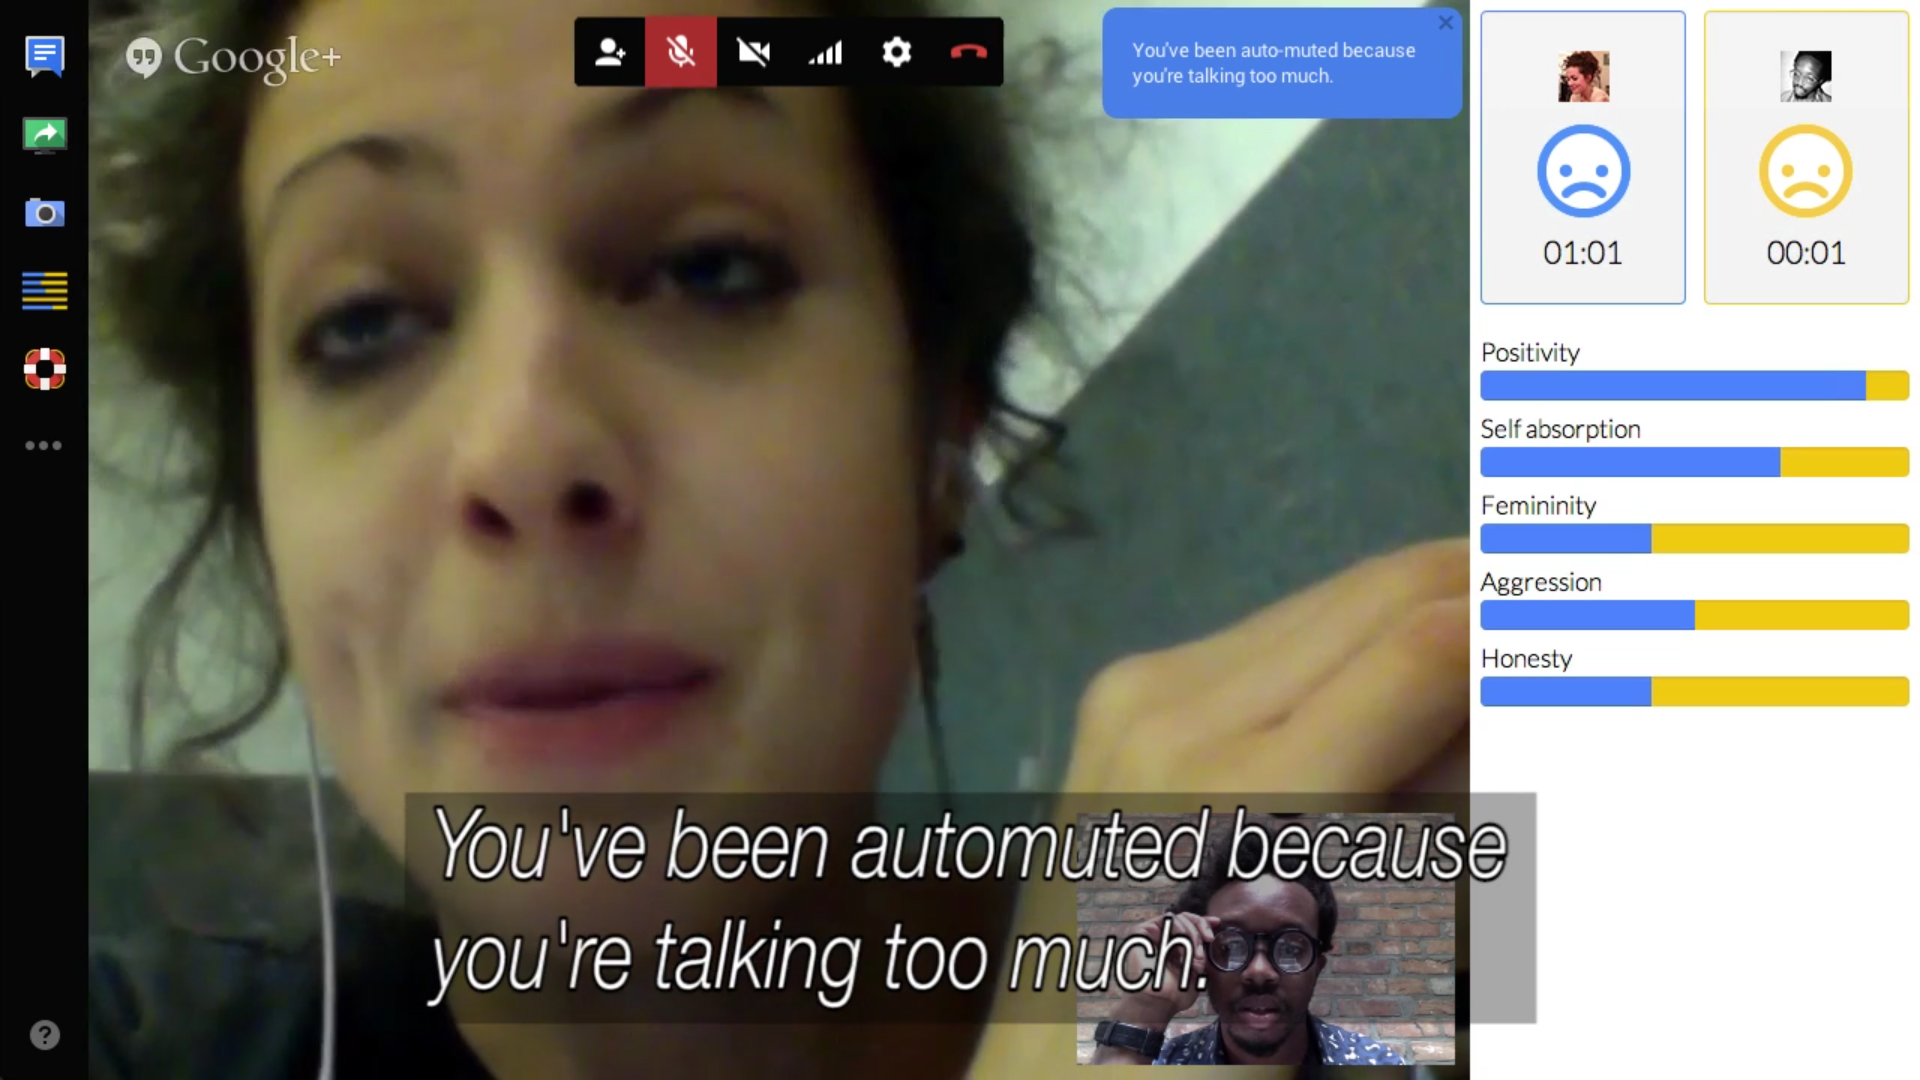
\includegraphics{./tex2pdf.9048/8a1224117ed91d8015226843bec5d97f13330fe4.jpg}

Bien que s'appuyant sur des études scientifiques similaires (analyse des
sentiments, comparaison des temps de parole) ces deux projets illustrent
deux manières d'aborder le sujet sensible de \emph{l'amélioration} des
compétences sociales grâce à la technologie. Le premier se revendique
comme \href{(https://www.youtube.com/watch?v=l3ztu9shfMg)}{une solution
presque thérapeutique} pour les gens qui ont des difficultés avec les
relations sociales, dans des différents contextes comme un entretien
d'embauche ou un rendez-vous galant. Derrière ce projet se trouve une
vision du comportement humain comme étant rationnel, quantifiable et
contrôlable grâce à des paramètres. Comme dans un jeu de gestion, on
doit atteindre son but (communiquer mieux) en ajustant différents
facteurs. Sauf que les règles qui régissent le ``monde réel'' sont plus
complexes, plus imprévisibles, et espérons-le, moins déterministes que
celles d'un jeu vidéo. À l'inverse, \emph{us+} se présente comme un
outil critique, soulignant la dépendance que l'on a envers des logiciels
hors de notre champ de compréhension, et ce même dans des aspects
intimes de notre vie comme dans nos communications
informelles.\footnote{Pour une critique plus approfondie d'us+, voir
  (``US+,'' n.d.).} C'est un projet qui est là pour poser la question
ouverte de la place et les limites que l'on souhaite donner à des
logiciels qui ont un contrôle grandissant sur la gestion de notre vie
quotidienne. C'est l'opposition entre une vision qui se pose la question
du \emph{comment} et une autre qui se pose celle du \emph{pourquoi}.

\newpage

\hypertarget{la-quuxeate-de-lefficacituxe9-la-quuxeate-de-la-singularituxe9}{%
\subsubsection{\texorpdfstring{\sout{La quête de l'efficacité} / La
quête de la
singularité}{La quête de l'efficacité / La quête de la singularité}}\label{la-quuxeate-de-lefficacituxe9-la-quuxeate-de-la-singularituxe9}}

Si le design doit viser à l'efficacité, alors on peut se poser la
question de la signification de ``communiquer efficacement''. De
nombreux outils nous font miroiter un ``discours optimisé'' :
\href{http://www.gingersoftware.com/fr}{\emph{Ginger}} promet à l'usager
``d'écrire mieux et plus vite'',
\href{http://www.hemingwayapp.com/}{\emph{Hemingway}} aide à produire
une écriture ``claire et audacieuse'', l'extension
\href{https://www.grammarly.com/}{\emph{Grammarly}} s'engage à la rendre
``claire, efficace et sans erreur''.

\begin{figure}
\centering
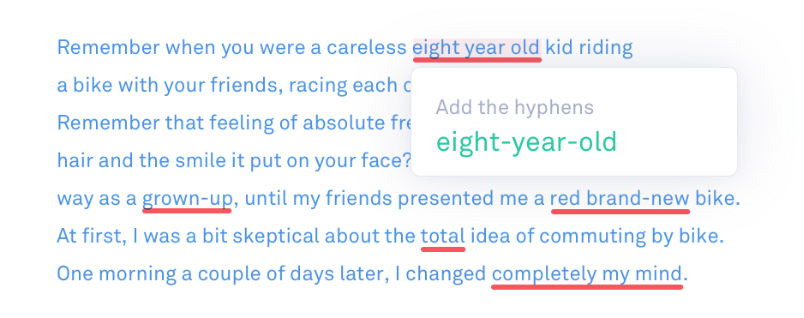
\includegraphics{./tex2pdf.9048/7e83c21e6796d91bba646886acdde75e134357da.jpg}
\caption{Grammarly souligne les mots ``problématiques''}
\end{figure}

Cette dernière, \emph{Grammarly}, est une application et une extension
pour navigateur qui souligne en temps réel les fautes d'orthographe, de
grammaire et de style. Ces corrections stylistiques incluent par exemple
la limitation des répétitions et la proposition de mots plus percutants
{[}\emph{compelling}{]}. Comme extension, elle peut superviser tout ce
que l'on écrit sur le web, des emails aux statuts sur les réseaux
sociaux. Chaque mot ``problématique'' est souligné, et une explication
sur le problème qu'il pose est accessible au survol. L'extension se
revendique comme un assistant pour l'écriture, promettant de la rendre
plus claire et communicative.

Le problème de l'optimisation promise par ces applications, c'est
qu'elle pousse à la standardisation en ramenant toutes les formes
d'écriture (email, statut) vers un mode argumentaire.

\begin{quote}
En fait la clarté est un attribut purement rhétorique, elle n'est pas
une qualité générale du langage, possible dans tous les temps et dans
tous les lieux, mais seulement l'appendice idéal d'un certain discours,
celui-là même qui est soumis à une intention permanente de persuasion.
{[}\ldots{}{]} Bien écrire -- désormais seul signe du fait littéraire --
c'est naïvement changer un complément de place, c'est mettre un mot ``en
valeur'', en croyant obtenir par là un rythme ``expressif''. Or
l'expressivité est un mythe : elle n'est que la convention de
l'expressivité. (Barthes 1953)
\end{quote}

Comme l'explique Barthes, la notion même de clarté ou d'expressivité
d'un discours n'est pas une propriété fondamentale du langage. C'est une
propriété héritée de la rhétorique, qui occulte d'autres aspects de la
communication, par exemple la spontanéité. La ``bonne manière de
parler'' est simplement une convention, qu'il est souvent bon de
connaitre, mais qui ne devrait pas être vue comme un but en soi. Ces
applications ont aussi une tendance à induire une confusion entre la
forme et le contenu. Elles présentent le contenu comme une matière
maléable qui peut se mouler dans des formes préétablies\footnote{Pour
  une analyse plus détaillée des systèmes de correction, voir (Christie
  2017).}.

Si l'argument de la ``communication efficace'' n'est pas univoque,
doit-on pour autant se désespérer de trouver un intérêt à la
conversation assistée par ordinateur ? La réponse se trouve peut-être
dans la capacité d'un logiciel à déranger les habitudes des usagers, et
c'est ce nous allons voir dans le prochain chapitre.

\newpage

\hypertarget{technologie-calme-technologie-perturbante}{%
\subsection{\texorpdfstring{\sout{technologie calme} =\textgreater{}
technologie
perturbante}{technologie calme =\textgreater{} technologie perturbante}}\label{technologie-calme-technologie-perturbante}}

La notion de ``technologie calme'' {[}\emph{calm technology}{]} est
introduite en 1995 par Mark Weiser et John Seely Brown dans le texte
\emph{Designing Calm Technology} (Weiser and Brown 1995). Ces deux
figures, occupant alors des postes à responsabilité au XEROX Parc, et
notamment Weiser, considéré comme le père de l'informatique ubiquitaire,
font le constat que les technologies de l'information sont de plus en
plus invasives et accaparent trop l'attention. Contre cette tendance,
ils expriment leur souhait d'une technologie calme, c'est-à-dire qui
n'accapare pas explicitement l'attention de l'utilisateur, et se situe
en périphérie de celui-ci.

Mais les auteurs ne proposent pas tant de limiter la place des systèmes
informatiques dans la vie quotidienne, ils proposent d'atténuer leur
présence en les rendant moins perceptibles. Ils ne questionnent pas tant
l'envahissement de la technologie, mais l'attention qu'elle recquière.

Nous verrons tout d'abord pourquoi l'idée d'une technologie qui
contraint l'usager peut être attrayante, puis nous remettrons en
question l'idée de reléguer la technologie en arrière-plan. Enfin, nous
verrons pourquoi ce n'est pas un problème de déranger l'usager avec des
détails techniques.

\newpage

\hypertarget{une-technologie-qui-fait-juste-ce-quon-lui-demande-une-technologie-qui-agit-luxe0-ouxf9-on-ne-lattend-pas}{%
\subsubsection{\texorpdfstring{\sout{Une technologie qui fait
\emph{juste} ce qu'on lui demande} / Une technologie qui agit là où on
ne l'attend
pas}{Une technologie qui fait juste ce qu'on lui demande / Une technologie qui agit là où on ne l'attend pas}}\label{une-technologie-qui-fait-juste-ce-quon-lui-demande-une-technologie-qui-agit-luxe0-ouxf9-on-ne-lattend-pas}}

Dans le chapitre précédent, nous évoquions les limites de la vision de
la technologie comme solution à la résolution d'un problème
{[}\emph{problem solver}{]}, et la vacuité de l'idée de ``communication
efficace''. De son côté, Weiser défend l'idée que les objets
électroniques ne devraient pas gêner des tâches pour lesquelles ils ne
sont pas mandatés. Et si, au contraire, on considérait qu'ils peuvent
nous surprendre en leur laissant de l'espace pour intervenir justement
là où on ne les attend pas ?

Tout designer a déjà entendu cette maxime à un moment de son parcours :
\emph{les contraintes sont créatives}. Ne pas avoir un outil
parfaitement adapté peut être agaçant, mais peut aussi pousser à
l'ingéniosité et générer des usages inattendus. Les contraintes obligent
à remettre en question ses habitudes et à imaginer des moyens créatifs
de les contourner. Des créations d'Oulipo au Conditional Design du
Studio Moniker (Maurer et al., n.d.), de nombreux artistes et designers
se sont appropriés la contrainte comme processus de création. Converser
par messagerie, c'est avant tout écrire, une activité créative qui a
toutes les raisons d'être réceptive à la contrainte. Les deux projets
présentés ci-dessous sont deux outils d'écriture atypiques qui utilisent
la contrainte comme point de départ.

Dans son projet \href{http://www.100x1000.net/}{\emph{100x1000}},
l'artiste Sterling Crispin propose d'écrire un court texte de cent mots
avec uniquement les mille mots les plus courants de la langue anglaise.
Si la personne saisis un mot qui n'appartient pas à ce corpus, il est
effacé aussitôt. Son programme donne un protocole d'écriture qu'il
serait épineux de suivre avec des moyens traditionnels comme une liste
imprimée de mots à vérifier. \emph{100x1000} autorise une forme
d'écriture qui ne serait pas envisageable sans l'outil informatique : il
en tire pleinement parti.

\href{http://www.themostdangerouswritingapp.com/}{\emph{The Most
Dangerous Writing App}} est une application web qui a pour but d'aider à
maintenir un rythme d'écriture soutenu. L'usager paramètre un temps
d'écriture (par exemple cinq minutes), durant lesquelles il doit écrire
en permanance. S'il arrête de saisir du texte pendant plus de cinq
secondes, tout le texte déjà tapé s'efface et est définitivement perdu.
Par un protocole un peu radical et presque un peu sadique, l'application
établit une situation d'écriture inédite. Il permet de trouver des
manières d'écrire qui ne seraient permises par un logiciel de traitement
de texte standard.

Ces projets sont deux exemples d'outils d'écriture qui utilisent la
contrainte comme prétexte pour encourager à écrire. Ce sont de petits
projets, au sens qu'ils ne sont pas complexes techniquement et qu'ils ne
peuvent servir que dans des situations particulières. Néanmoins, ils
permettent d'entrevoir la pluralité des expériences que pourraient
proposer des logiciels de traitement de texte revisités.

\newpage

\hypertarget{une-technologie-qui-agit-en-arriuxe8re-plan-une-technologie-explicitement-paramuxe9trable}{%
\subsubsection{\texorpdfstring{\sout{Une technologie qui agit en
arrière-plan} / Une technologie explicitement
paramétrable}{Une technologie qui agit en arrière-plan / Une technologie explicitement paramétrable}}\label{une-technologie-qui-agit-en-arriuxe8re-plan-une-technologie-explicitement-paramuxe9trable}}

Une notion au centre de la \emph{calm technology} est celle de
``périphérie''. Weiser recommande de concevoir des objets électroniques
qui sont présents de manière ambiante\footnote{C'est la vision à la base
  de la notion d'informatique ubiquitaire, que Weiser a contribué à
  définir et populariser. Voir
  http://www.ubiq.com/hypertext/weiser/UbiHome.html}, et qui
s'approprient le moins possible l'attention explicite de l'utilisateur.
Une illustration de cette idée est celle du thermostat, qui une fois
configuré ne nécessite plus d'intervention pour maintenir la température
souhaitée, ou encore le coffre de la voiture qui s'ouvre avec un simple
mouvement de la jambe. Concrètement, un moyen souvent évoqué est de
recourir à des capteurs, qui vont recueillir des informations ``en
arrière plan'', et ainsi laisser à l'usager toute son attention. Les
deux prochains chapitres expliquent pourquoi cette idée n'est pas
compatible avec l'utilisation massive de données personnelles.

\hypertarget{fais-ce-que-je-dis-pas-ce-que-je-fais}{%
\paragraph{Fais ce que je dis, pas ce que je
fais}\label{fais-ce-que-je-dis-pas-ce-que-je-fais}}

La personnalisation, dans le sens de l'adaptation d'un système aux
habitudes de l'utilisateur, élément clé des systèmes de recommandation,
repose précisement sur cette idée. Ces derniers se nourrissent de notre
comportement quotidien implicite, comme retenir les mots employés
fréquement pour nous les proposer par la suite, ou encore identifier les
contacts desquels nous sommes le plus proches pour nous suggérer qui est
en ligne. Toujours en quête de métadonnées à analyser, ils considèrent
des actions inconscientes comme des choix manifestes.

\begin{quote}
In other words, how are we to deal with a common problem faced by
parents who often say to their children, \emph{Don't do what I do; do
what I say} ? Obviously while learning by observation is a good way to
learn about things in the world and actions to take in certain contexts,
it is not enough to actually know why you are taking an action, or when
you should take an action. (Hendler and Mulvehill (auth.) 2016, 158)
\end{quote}

Cependant, comme le souligne Hendler dans son ouvrage sur ce qu'il
appelle les ``machines sociales'', que ce soit par manque d'expérience
ou par erreur de jugement, on est tous amené à faire des actions que
l'on n'approuve pas tout à fait ou que l'on ne considère pas comme nous
représentant réellement. Entre ce que je suis, ce que je fais, et ce que
je voudrais être, il y a des écarts qui peuvent être lourds de
signification. Or la personnalisation ne prend pas en compte ces
contradictions qui font partie du comportement humain. Le système voit
ainsi ses usagers sous une identité simplifiée, caricaturale, pour des
raisons qui peuvent être au mieux techniques, au pire tout à fait
idéologiques\footnote{On peut penser par exemple à Mark Zuckerberg, qui
  déclarait en 2011 à David Kirkpatrick dans \emph{The Facebook Effect}
  (Simon \& Schuster) qu'avoir deux identités était un exemple de
  ``manque d'intégrité''.}. C'est là un enjeu de la personnalisation :
comment faire le tri entre les actions qui sont signifiantes et celles
qui ne le sont pas, et qui peuvent même être contradictoires avec la
personnalité réelle d'un individu.\\

C'est pourquoi un point primordial à considérer est celui de concéder à
l'usager le contrôle sur son identité. Cela impose de ne plus avoir une
personnalisation autosuffisante, mais guidée par l'usager lui-même. Il
s'agit donc de promouvoir des systèmes hybrides, qui combinent les
données collectées avec les injonctions explicites de l'utilisateur
final.

\newpage

\hypertarget{ne-pas-en-dire-trop-sur-comment-le-systuxe8me-fonctionne-dire-clairement-comment-le-systuxe8me-fonctionne}{%
\subsubsection{\texorpdfstring{\sout{Ne pas en dire trop sur comment le
système fonctionne} =\textgreater{} Dire clairement comment le système
fonctionne}{Ne pas en dire trop sur comment le système fonctionne =\textgreater{} Dire clairement comment le système fonctionne}}\label{ne-pas-en-dire-trop-sur-comment-le-systuxe8me-fonctionne-dire-clairement-comment-le-systuxe8me-fonctionne}}

Nous venons de voir qu'il faut relativiser les données récupérées sur
les usagers, car elles peuvent être loin de représenter leur
personnalité. Mais parfois, l'effet inverse peut se produire : elles
peuvent traduire des détails sensibles sur notre vie.

Ces données ``personnelles'' peuvent être les informations que l'on
saisit soi-même sur ses profils de réseaux sociaux, comme l'âge, le lieu
de vie ou la profession. Elles peuvent également être des indications
sur le comportement d'utilisation, par exemple les personnes avec
lesquelles on parle souvent, ou encore les heures de fréquentation d'une
application. Ces données comportementales, nous avons tendance à oublier
que nous les cédons gracieusement contre la gratuité de services comme
Google ou Facebook.\footnote{``Nous recueillons des informations sur les
  personnes et les groupes avec lesquels vous êtes en contact, ainsi que
  la manière dont vous interagissez avec eux (par exemple, les personnes
  avec qui vous communiquez le plus ou encore les groupes au sein
  desquels vous aimez vous exprimer)'', ``Nous recueillons également des
  informations concernant la manière dont vous utilisez nos Services,
  telles que {[}\ldots{}{]} la fréquence et la durée de vos activités.''
  Voir la
  \href{https://www.facebook.com/privacy/explanations}{\emph{Politique
  d'utilisation des données}} de Facebook.} Or, elles trahissent des
aspects intimes de notre vie. On ne sait pas avec exactitude comment
toutes ces données sont utilisées, il est donc difficile d'estimer
quelles informations sont sensibles. Mais de telles quantités de données
peuvent traduire plus qu'on ne pourrait l'imaginer. L'écrivaine Joanne
McNeil évoque par exemple comment les ``souhaits d'anniversaire''
{[}\emph{birthday wishes}{]} sur Facebook pourraient être des
indicateurs de la proximité affective que l'on a avec un ``ami'' (McNeil
2014), et donc rapporter directement de l'argent à l'entreprise. Ces
conclusions sont difficilement vérifiables, et pourtant elles sont loin
d'être improbables. Je suis plus attentive à une annonce pour des
cadeaux à l'approche de l'anniversaire de mon meilleur ami, comme je le
serais plus à l'approche des fêtes de fin d'année. Et pour une
entreprise qui gagne de l'argent grâce à la vente d'espace publicitaire,
c'est une aubaine.

Dès lors, on peut interpréter de la même manière les fonctions de
réponse automatique (que l'on peut considérer comme une forme
d'autocomplétion) inclues dans Gmail. Dans la situation (réelle)
présentée ici, quelle différence de sens y a-t-il entre ``I don't have
it.'' et ``I don't, sorry.'', si ce n'est que la première est plus
sèche, et la seconde plus aimable ? Si je choisis la première, mon
interlocuteur sera-t-il interprété comme un collègue que je n'apprécie
pas trop ? Et si je choisis la deuxième, sera-t-il considéré comme une
personne avec laquelle j'ai des relations amicales ?

\begin{figure}
\centering
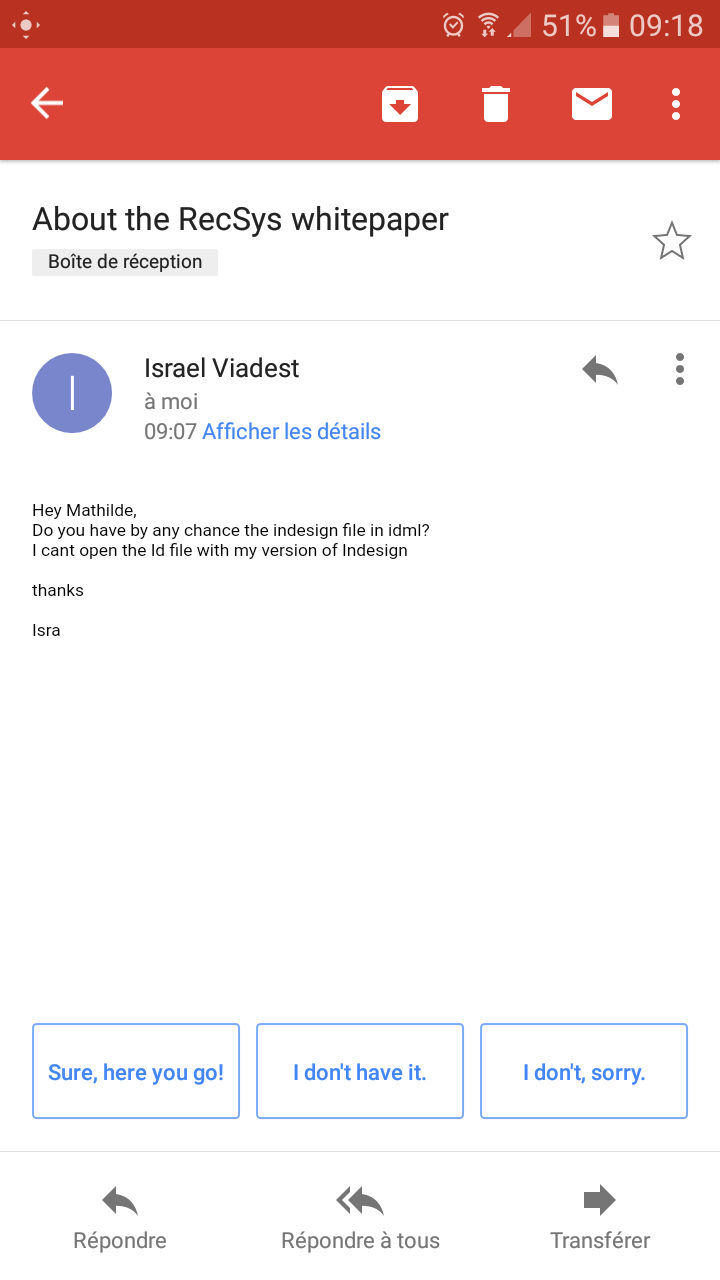
\includegraphics{./tex2pdf.9048/e4033b915be97c761b70f61e61fe759c2920db99.png}
\caption{``Salut Mathilde, est-ce que tu as le fichier indesign en
format idml ?'' -\textgreater{} ``Oui, le voici !'' \textbar{} ``Non, je
ne l'ai pas.'' \textbar{} ``Je ne l'ai pas, désolé.''}
\end{figure}

On pourrait aller encore plus loin et spéculer sur ce qui pourrait être
connu de nous dans le cas de l'analyse de conversations privées sur une
application comme Messenger. La fréquence des contacts, l'usage de mots
particuliers ou de smileys sont autant de facteurs qui révèlent avec
précision la nature de la relation entre deux personnes (familiale,
amicale, amoureuse\ldots{}).

Un entreprise comme Google ne communique pas avec précision sur
\emph{comment} elle les utilise nos données, et pourtant c'est grâce à
elles qu'elle gagne de l'argent. De ce point de vue, être en mesure de
pouvoir les consulter, connaître leurs implications, les modifier et les
supprimer de manière simple répond à une question d'éthique.

De ce point de vue, l'idée d'une technologie qui capte en arrière-plan
des informations sur ses usagers est problématique.

\newpage

\hypertarget{design-invisible-design-visible}{%
\subsection{\texorpdfstring{\sout{design invisible} =\textgreater{}
design
visible}{design invisible =\textgreater{} design visible}}\label{design-invisible-design-visible}}

\hypertarget{la-meilleure-interface-est-pas-dinterface}{%
\paragraph{``La meilleure interface est\ldots{} pas
d'interface''}\label{la-meilleure-interface-est-pas-dinterface}}

Nous venons de voir les problèmes que peut soulever l'idée de calm
technology, notamment dans le cadre de systèmes manipulant des données
personnelles. Souvent affiliée sur le plan idéologique avec l'idée de
``calm technology'', la notion de ``design invisible'' ou le mouvement
\emph{NoUI} (littéralement \emph{pas d'interface utilisateur}),
nouvellement popularisés par des ouvrages comme \emph{The Best Interface
is No Interface} (Krishna 2015), sont plusieurs termes qui désignent une
même tendance : celle selon laquelle le bon design est celui qui ne se
voit pas, celui qui génère le moins de friction possible avec
l'utilisateur\footnote{On peut également citer \emph{The Invisible
  Computer} de Don Norman, publié en 1998.}. Ce mouvement considère
l'interface graphique {[}\emph{GUI, Graphical User Interface}{]} comme
une couche additionnelle à l'expérience utilisateur, et qui est souvent
superflue.

Or, la multiplication des assistants personnels et la prolifération
d'outils de \emph{quantified self} oriente de manière significative nos
prises de décisions. Ces assistants ne nous disent pas quoi faire, pas
plus qu'ils ne décident à notre place, mais l'on se repose de plus en
plus sur eux pour ordonner notre vie de tous jours. Pour cette raison,
la compréhension du système par les usagers est primordiale et une
interface visible est une étape clé dans l'élaboration de cette
``médiation technique''.

Ce mouvement est régulièrement critiqué. On peut par exemple citer Timo
Arnall\footnote{(Arnall 2013).} ou Dave Hall\footnote{(Hall 2017).} pour
les articles critiques qu'ils ont publiés à ce sujet. Ici, nous allons
voir tout d'abord questionner un principe du mouvement NoUI ``Tirer
parti des ordinateurs au lieu de les servir'', en présentant les
bénéfices d'une adaptation de l'usager à la logique computationnelle.
Puis nous expliquerons pourquoi l'idée d'invisibilité est
particulièrement problématique dans l'ère du machine learning.

\newpage

\hypertarget{tirer-parti-des-ordinateurs-plutuxf4t-que-de-les-servir-sadapter-uxe0-la-logique-computationnelle}{%
\subsubsection{\texorpdfstring{\sout{Tirer parti des ordinateurs plutôt
que de les servir} =\textgreater{} S'adapter à la logique
computationnelle}{Tirer parti des ordinateurs plutôt que de les servir =\textgreater{} S'adapter à la logique computationnelle}}\label{tirer-parti-des-ordinateurs-plutuxf4t-que-de-les-servir-sadapter-uxe0-la-logique-computationnelle}}

Parmi les principes évoqués dans \emph{The Best Interface is No
Interface}, il y a celui selon lequel ce n'est pas aux humains de
s'adapter aux ordinateurs, mais aux ordinateurs de s'adapter aux
humains. Et si, à l'inverse, encourager les usagers à s'adapter à leurs
outils, c'était leur donner la capacité de mieux les comprendre et de
construire les conditions nécessaires à une appropriation plus forte de
la technologie par les gens qui la côtoient au quotidien ?

Pour illustrer son propos, Krishna prend l'exemple du remplissage de
formulaires en ligne. Il évoque ce moment agaçant, quand on ajoute des
tirets, des espaces ou des points entre les nombres de notre numéro de
téléphone, et que le système nous indique par un message d'erreur qu'il
ne doit contenir que des chiffres. Selon lui, il faut créer des systèmes
qui savent reconnaître et interpréter ces ``erreurs'', de manière à ne
pas ennuyer l'utilisateur avec des détails techniques, qui n'ont de sens
que pour la machine.

Néanmoins, contraindre l'usager à parler à l'ordinateur dans son
langage, lui demander de s'adapter à son mode de compréhension, génère
une connaissance plus juste de la réalité des capacités techniques des
ordinateurs. Quand je rentre mon numéro de téléphone, mon ordinateur ne
sait pas comment m'appeler, il ne fait qu'associer une suite de nombres
à mon profil, sous le label ``téléphone''. M'obliger à ne pas inclure
d'espace quand je saisis mon numéro, c'est me rappeler que ce n'est pas
mon numéro de téléphone que l'ordinateur comprend, mais bien une série
de chiffres.

La nuance est mince, mais contribue à alimenter une incompréhension de
la technologie par les gens qui l'utilisent pourtant au quotidien. Or,
une technologie incomprise génère de la frustration et restreint la
créativité. Une étude conduite il y a déjà une dizaine d'années montre
que les problèmes posés par une mauvaise compréhension de la technologie
incluent : de mauvaises suppositions sur les risques d'adoption de cette
technologie; des attentes en terme de bénéfices qui sont en décalage
avec la réalité des possibilités techniques; des difficultés à trouver
des solutions quand intervient un problème avec celle-ci (Poole et al.
2008). Il cite l'exemple d'une personne qui pensait que les RFID étaient
des traqueurs de position. Cette croyance populaire (que les auteurs
nomment en anglais \emph{folk theories}) le faisait s'inquiéter que des
vendeurs ou des organisations gouvernementales utilisent des
technologies basées sur le RFID pour l'espionner. Cette situation
illustre comment un malentendu sur son fonctionnement peut avoir des
conséquences considérables sur l'adoption d'une technologie. De plus,
l'étude conclue que, même s'ils portent en eux de sérieuses inquiétudes
face aux nouvelles technologies, les participants étaient réticents à
faire remonter publiquement leurs doutes. Une des raisons avancées est
qu'ils doutent de leur possibilité d'avoir leur mot à dire dans une
évolution technologique qu'ils perçoivent comme inévitable.

\begin{quote}
By removing our knowledge of the glue that holds the systems that make
up the infrastructure together, it becomes much more difficult, if not
impossible, to begin to understand how we are constructed as subjects,
what types of systems are brought into place (legal, technical, social,
etc.) and where the possibilities for transformation exist (Ratto 2007).
\end{quote}

Sur le même sujet, Matt Ratto souligne qu'une incompréhension de la
technologie rend difficile, voir impossible une réflexion sur les
possibilités de transformation de celle-ci. En ne montrant pas le
fonctionnement d'un système, on retire aux gens leur abilité à le
comprendre, le critiquer et le reconfigurer, c'est-à-dire leur abilité à
imaginer que les choses soient différentes. Vu sous cet angle, le design
``invisible'' participe à creuser un fossé entre les professionnels qui
créent des ces objets électroniques et les personnes qui les utilisent.
On voit que les conclusions que l'étude témoignent d'un imaginaire
technologique limité chez les usagers (mauvaise estimation des
possibilités techniques, difficulté d'improviser en cas de problème).
Dans ce contexte, donner les clés de compréhension d'un système en
demandant une adaptation des usagers à la logique computationnelle
rendrait possible un renouvellement de cet imaginaire. Les objets
électroniques et les logiciels ne devraient pas être vus uniquement
comme complexes (même s'ils le sont indéniablement), ni comme une
matière figée, mais au contraire comme des entités en permanente
évolution, questionnables, et qui peuvent être modelées de manière
collaborative (Finn 2017, 7).

\newpage

\hypertarget{la-magie-de-linvisibilituxe9-la-nuxe9cessituxe9-de-visibilituxe9}{%
\subsubsection{\texorpdfstring{\sout{La magie de l'invisibilité}
=\textgreater{} La nécessité de
visibilité}{La magie de l'invisibilité =\textgreater{} La nécessité de visibilité}}\label{la-magie-de-linvisibilituxe9-la-nuxe9cessituxe9-de-visibilituxe9}}

Les modèles statistiques à la base des algorithmes de machine learning
parviennent, par l'analyse de grandes quantités de données, à souligner
des corrélations invisibles pour un humain ordinaire. Ces liens
mystérieux sont fascinants, ils captivent, bien qu'ils ne soient pas une
source de connaissance explicable. A titre d'exemple, on peut penser aux
\href{(https://informationisbeautiful.net/2010/peak-break-up-times-on-facebook/)}{``pics
de rupture''}, représentés par David McCandless \& Lee Byron, appuyés
sur les mises à jour de statut Facebook, qui montrent une hausse au
début du printemps et deux semaines avant Noël{[}\^{}5ee2{]}. Quelle
explication donner à ce phénomène ? Difficile à dire. Si l'on peut
s'amuser à faire des suppositions, il faut garder à l'esprit que ce ne
sont que des hypothèses.

\hypertarget{duxe9celer-les-dysfonctionnements}{%
\paragraph{Déceler les
dysfonctionnements}\label{duxe9celer-les-dysfonctionnements}}

Pour illustrer cette problématique, on peut se pencher sur une étude
exposant le problème posé par une faible intelligibilité des modèles
basés sur du machine learning. ``L'intelligibilité'' correspond à la
capacité à comprendre pourquoi le système prend une décision.\\
Cette étude se place dans le cadre de services de santé. Son but était
de concevoir un modèle capable de déterminer les patients avec une haute
probabilité de décès (PDD) par pneumonie de manière à les hospitaliser,
et traiter ceux avec une faible probabilité en consultation externe
(Caruana et al. 2015)\footnote{Pour une analyse de cette étude voir
  (Manny 2017).}. Deux modèles sont envisagés : un basé sur des réseaux
de neurones {[}\emph{neural networks}{]}, avec une précision plus élevée
mais jugé trop risqué, et un second, basé sur des règles, moins précis,
et qui sera choisi en définitive. Sans entrer dans des détails
techniques\footnote{Pour une explication plus approfondie de pourquoi
  des réseaux de neurones sont opaques par nature (McQuillan 2017).}, ce
second modèle permet explicitement, à l'inverse du premier, de voir les
relations entre entre chaque valeur analysée et la PDD associée. Il
révèle par exemple que, statistiquement, être asthmatique est corrélé
avec un faible niveau de PDD. À première vue, c'est une observation
illogique. En fait, il s'avère que les patients atteints de pneumonie
avec des antécédents asthmatiques sont généralement expédiés en unité de
soins intensifs. Comme le pronostic pour ces patients est meilleur que
la moyenne, leur chance de survie l'est aussi. Ainsi, la corrélation
existe, mais il n'y pas de lien de causalité. Malgré sa puissance de
calcul, l'analyse statistique ne différencie pas la réelle bonne
performance du système médical et une supposée robustesse de la santé du
patient. Si le modèle basé sur le réseau de neurones avait été choisi,
il aurait pu délibérement suggérer d'envoyer un patient asthmatique en
consultation externe au lieu des urgences. Cet exemple illustre la
nécessité de ne pas avoir une confiance absolue dans des algorithmes
dont on n'est pas en mesure de comprendre le fonctionnement.\footnote{Pour
  une analyse plus détaillée, et des propositions concrètes sur comment
  rendre visible une décision est automatisée, voir (Sheret 2017).}

Dans un système d'autocomplétion basé sur du machine learning, une
dérive pourrait par exemple se trouver si certaines associations
statistiques de mots étaient révélatrices de préjugés. Par exemple, si
les adjectifs associés à un pronom féminin étaient différents de ceux
associés à un pronom masculin, et traduisaient une tendance à qualifier
les femmes par leur physique et les hommes par leurs capacités. Ce ne
serait pas un biais causé par le système d'autocomplétion, mais un biais
qui existe dans le monde réel (Bian, Leslie, and Cimpian 2017) et qui
serait ainsi prolongé. Grâce à une visibilité sur de telles
corrélations, il est possible d'établir des rééquilibrages pour
favoriser certains aspects de la langue. C'est par exemple le constat à
l'origine d'une application de clavier initée par Plan International, le
\href{https://sheboard.com/}{sheboard} (``A Mobile Keyboard by Plan
International Boosts Girls' Confidence,'' n.d.). Ce clavier a pour
spécificité un système d'autocomplétion qui suggère des mots issus de
champs lexicaux qui vont contre les préjugés que l'on porte envers les
femmes.

\begin{figure}
\centering
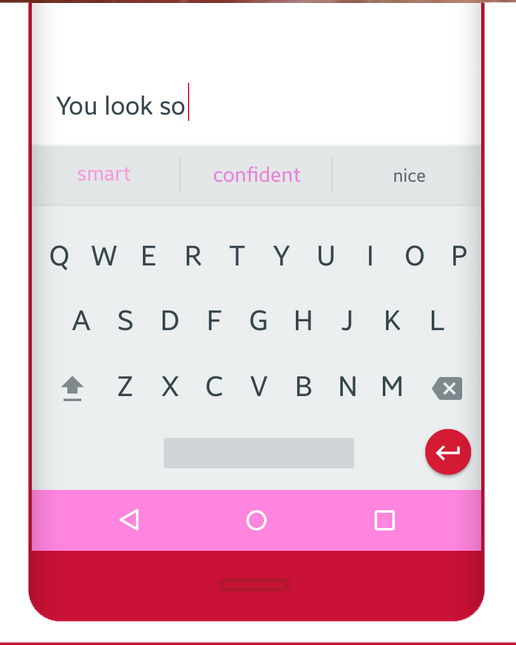
\includegraphics{./tex2pdf.9048/f435c928828e24e11182ac7a78fd5f70dda7e6a3.png}
\caption{Le système d'autocomplétion de Sheboard est conçu de telle
manière à favoriser l'association de noms féminins avec un champ lexical
de la réussite et de la confiance en soi}
\end{figure}

En ayant une visibilité sur comment les suggestions sont produites, on
offre la possibilité de relativiser des résultats inappropriés, et
d'élaborer des stratégies pour leur faire face.

\newpage

\hypertarget{vers-de-nouvelles-formes-de-collaboration-humain-machine}{%
\subsection{Vers de nouvelles formes de collaboration
humain-machine}\label{vers-de-nouvelles-formes-de-collaboration-humain-machine}}

Au cours des trois chapitres précédents, nous avons vu comment les
logiciels changent, et pourraient changer notre manière d'interagir via
la parole et l'écriture. Nous avons également vu quelles habitudes de
conceptions instaurer pour tenir compte des spécificités des expériences
basées sur des algorithmes. Ces habitudes s'articulent autour de trois
points clés : en premier lieu, pousser à l'inventivité en priviliégiant
une approche critique et en valorisant des usages insolites sur la
résolution d'un problème. En second lieu . Et enfin, expliquer le
fonctionnement du système grâce à une interface qui montre l'envers du
décor.

Dans cette dernière partie, qui sert de conclusion, nous élargirons le
sujet sur la relation humain-machine en questionnant l'idée d'assistant
personnel et en désignant la modularité et la paramétrabilité d'un
logiciel comme des caractéristiques essentielles. Puis nous définirons
l'idée de \emph{technologie chili} comme une synthèse des points évoqués
dans les chapitres précédents.

\hypertarget{la-technologie-en-tant-quoutil-cruxe9atif-dexpression-et-non-en-temps-quassistant}{%
\subsubsection{La technologie en tant qu'outil créatif d'expression et
non en temps
qu'assistant}\label{la-technologie-en-tant-quoutil-cruxe9atif-dexpression-et-non-en-temps-quassistant}}

Les principes évoqués précédemment doivent nous amener à regarder les
objets électroniques sous un regard qui n'est peut-être pas celui d'un
\emph{assistant}. Est-on obligé de penser l'assistance sous l'angle
d'une visée utilitariste ? N'y aurait-il pas des alternatives ?

L'imaginaire que l'on associe aux ``assistants personnel'' est influencé
par une vision anthropomorphique de l'intelligence artificielle. Comme
nous l'avons évoqué dans l'introduction avec le test de Turing et ELIZA,
on a tendance à considérer qu'un ordinateur intelligent est un
ordinateur qui se comporte comme un humain : qui est capable de parler,
écrire, être émotif. Mais les appareils électroniques peuvent avoir un
intérêt au-delà de cette image de l'humain ``augmenté''. On peut voir
l'autocomplétion non pas comme un assistant mais comme un \emph{outil
créatif}.\\
Le terme d'asssitant induit une relation hiérarchique, un assistant nous
est subordonné. Il est celui auquel on délègue une tâche, qu'on est
souvent en mesure de réaliser, mais qu'on n'a pas envie de faire.
Pourquoi ne pas penser cette relation plutôt comme une forme de
collaboration ?

\hypertarget{limportance-davoir-des-logiciels-paramuxe8trables-et-modulaires}{%
\subsubsection{L'importance d'avoir des logiciels paramètrables et
modulaires}\label{limportance-davoir-des-logiciels-paramuxe8trables-et-modulaires}}

Comme dans une équipe, la compréhension mutuelle entre les deux
équipiers est un facteur déterminant pour le succès d'une collaboration.
Elle peut passer, comme nous l'avons vu dans la partie 4, par une
interface qui laisse transparaître le fonctionnement du système. Mais
elle peut aussi passer par des logiciels modulaires et aisément
paramétrables, permettant des possibilités d'usage exponentielles. Par
\emph{modulaire} j'entends un logicel sur lequel on peut venir des
greffer d'autre petits logiciels, de manière enrichir ses
fonctionnalités. Par \emph{paramétrable} j'entends des possibilités de
configuration étendues. Ces deux directions encouragent une diversité
des fonctionnalités en laissant aux usagers eux-mêmes la possibilité de
personnaliser leurs outils.

\begin{quote}
Ainsi, ce que dénonce David M. Berry, c'est bien le développement de
certains types de machines (programmes) avec lesquelles nous ne pouvons
strictement rien faire, ou peu faire, ou ne rien faire qui n'ait déjà
été anticipé -- des machines qui « rendent service » de façon si
parfaitement programmée qu'aucune marge de manoeuvre ne sera possible,
mettant ainsi en défaut toute conduite technique. Contre
l'automatisation issue des sciences comportementales, il nous faut donc
oeuvrer à rechercher et à créer des « marges d'indétermination » au sein
de nos rapports aux machines. (Masure 2016)
\end{quote}

Comme le souligne Anthony Masure, la collaboration humain-machine ne
doit pas passer par des machines qui seraient de plus en plus autonomes
et ne laissent pas de marge de manoeuvre à l'usager; mais au contraire
par des machines plus facilement manipulables. Si l'on commence à penser
les ``assistants'' non pas comme des logiciels parfaitement conçus, à
utiliser selon des critères prédéfinis, mais comme une base pouvant être
étendue à l'infini par l'usager, alors on laisse une place à des usages
originaux et inventifs.

\hypertarget{le-moduxe8le-des-extensions}{%
\subsubsection{Le modèle des
extensions}\label{le-moduxe8le-des-extensions}}

Un modèle qui tire parti de cette modularité est celui des extensions
{[}\emph{addons}{]} pour navigateurs (Firefox ou Google Chrome par
exemple). Une extension est un petit programme qui enrichit les
fonctionnalités d'un navigateur. Ce n'est pas un logiciel ni une
application en soit, mais un module que l'on peut greffer sur un
logiciel existant pour étendre ses fonctions. Certaines extensions sont
officielles et grand public (bloqueurs de publicité, calendriers,
traducteurs). D'autres ressemblent plus à de petits
\emph{hacks}\footnote{Un hack est une solution rapide, bricolée mais
  ingénieuse pour contourner un problème (``The Original Hacker's
  Dictionary,'' n.d.).}, par exemple \emph{I'm not robot captcha
clicker} valide le captcha à la place de l'usager pour lui faire gagner
quelques secondes, ou bien \emph{Disable Ctrl-Q} empêche de fermer son
navigateur par accident avec le raccourci clavier `ctrl+Q'. D'autres
enfin sont des projets artistiques, voir activitistes, par exemple
\href{http://lovemachine.cc/}{loveMachine}, qui envoie un ``j'aime'' à
toutes les publications disponibles dans le fil d'actualité de Facebook
pour compliquer la tâche des entreprises faisant de la publicité
ciblée.\\
Les extensions peuvent provenir de sources variées, de développeurs
professionnels comme amateurs, ce qui les rend porteuses d'une diversité
impossible à trouver dans un logiciel classique.

\hypertarget{une-technologie-chili}{%
\subsubsection{Une technologie chili}\label{une-technologie-chili}}

En conclusion, je souhaiterais définir l'idée d'une technologie
``chili'', comme alternative à celles évoquées dans les chapitres
précédents.\\
Hélas, je ne considère pas que le monde de l'art et du design manque de
termes spécialisés dont l'utilité est doûteuse (Jacobi 2005)\footnote{Voir
  (Feron, n.d.).}. Cependant, il y a un an, quand j'ai commencé à
définir mon sujet de mémoire, j'essayais en vain de l'articuler autour
de la question de ``comment les assistants personnels peuvent pimenter
les relations sociales ?''. Je tentais de le formuler différemment, mais
cette idée de ``piment'' me restait toujours dans la tête. C'est alors
que je suis tombée face à cette conférence de Frédéric Kaplan, vieille
de déjà dix ans (Kaplan 2007). Il présente durant une vingtaine de
minutes différentes expérimentations mettant en scène AIBO, un
robot-chien (ou chien-robot ?) de compagnie, développé par Sony et à la
conception duquel il a contribué. Ces différentes expériences mettent en
lumière les \emph{relations} de curiosité, de peur ou de complicité qui
se créent entre le robot et l'environnement dans lequel il est déployé :
les enfants, les autres animaux de compagnie ou le maître qui cherche à
lui apprendre à reconnaître une balle. Pour conclure sa présentation il
évoque l'idée d'une ``technologie chili'', qu'il place antipodes d'une
technologie calme.

\begin{quote}
Maybe you want \emph{chili technology}, maybe you actually think that
technology is something a bit exciting that should push you a little
bit. Not just being in the background and do just what you want to do,
but sometimes, come in your life and have a kind of unexpected effect.
\end{quote}

Il définit ce type de technologie par sa capacité à être un peu
excitante, à surprendre et à faire naître des situations inattendues.
Une forme de technologie qui ne viendrait pas seulement résoudre un
problème, mais agrémenter la vie de tous les jours. C'est autour de
cette base et des principes évoqués dans les chapitres précédents que se
définissent les principes suivants.

\newpage

\hypertarget{technologie-chili}{%
\subsubsection{Technologie chili}\label{technologie-chili}}

\hypertarget{un-objectif-pousser-uxe0-linventivituxe9}{%
\paragraph{Un objectif : pousser à
l'inventivité}\label{un-objectif-pousser-uxe0-linventivituxe9}}

L'intérêt d'une technologie ne se résume pas à solutionner des
problèmes. Elle permet de créer un espace pour la pensée associative et
la curiosité.

\hypertarget{une-expuxe9rience-perturbante}{%
\paragraph{Une expérience
perturbante}\label{une-expuxe9rience-perturbante}}

Un système automatisé n'agit pas en arrière-plan. Il pousse l'usager à
se dépasser, apprend de lui et lui fait front.

\hypertarget{une-interface-visible}{%
\paragraph{Une interface visible}\label{une-interface-visible}}

L'interface n'est ni une couche d'embellissement, ni une couche
accessoire. Elle doit donner les clés de compréhension du fonctionnement
du système.

\newpage

\hypertarget{annexe-et-si}{%
\subsection{Annexe : Et si\ldots{} ?}\label{annexe-et-si}}

Toute au long de ce mémoire, j'ai défendu plusieurs principes pour la
conception de l'expérience et l'interface d'un système d'autocomplétion.

En parallèle, en temps que designer, il me paraissait important
d'illustrer ces principes par des exemples d'application. Cette annexe
présente une petite collection d'interfaces fictionnelles, qui tirent
parti des algorithmes de machine learning, en se plaçant dans la lignée
de la technologie chili.

\newpage

\hypertarget{coach-personnel-pour-les-relations-sociales}{%
\subsubsection{Coach personnel pour les relations
sociales}\label{coach-personnel-pour-les-relations-sociales}}

\begin{figure}
\centering
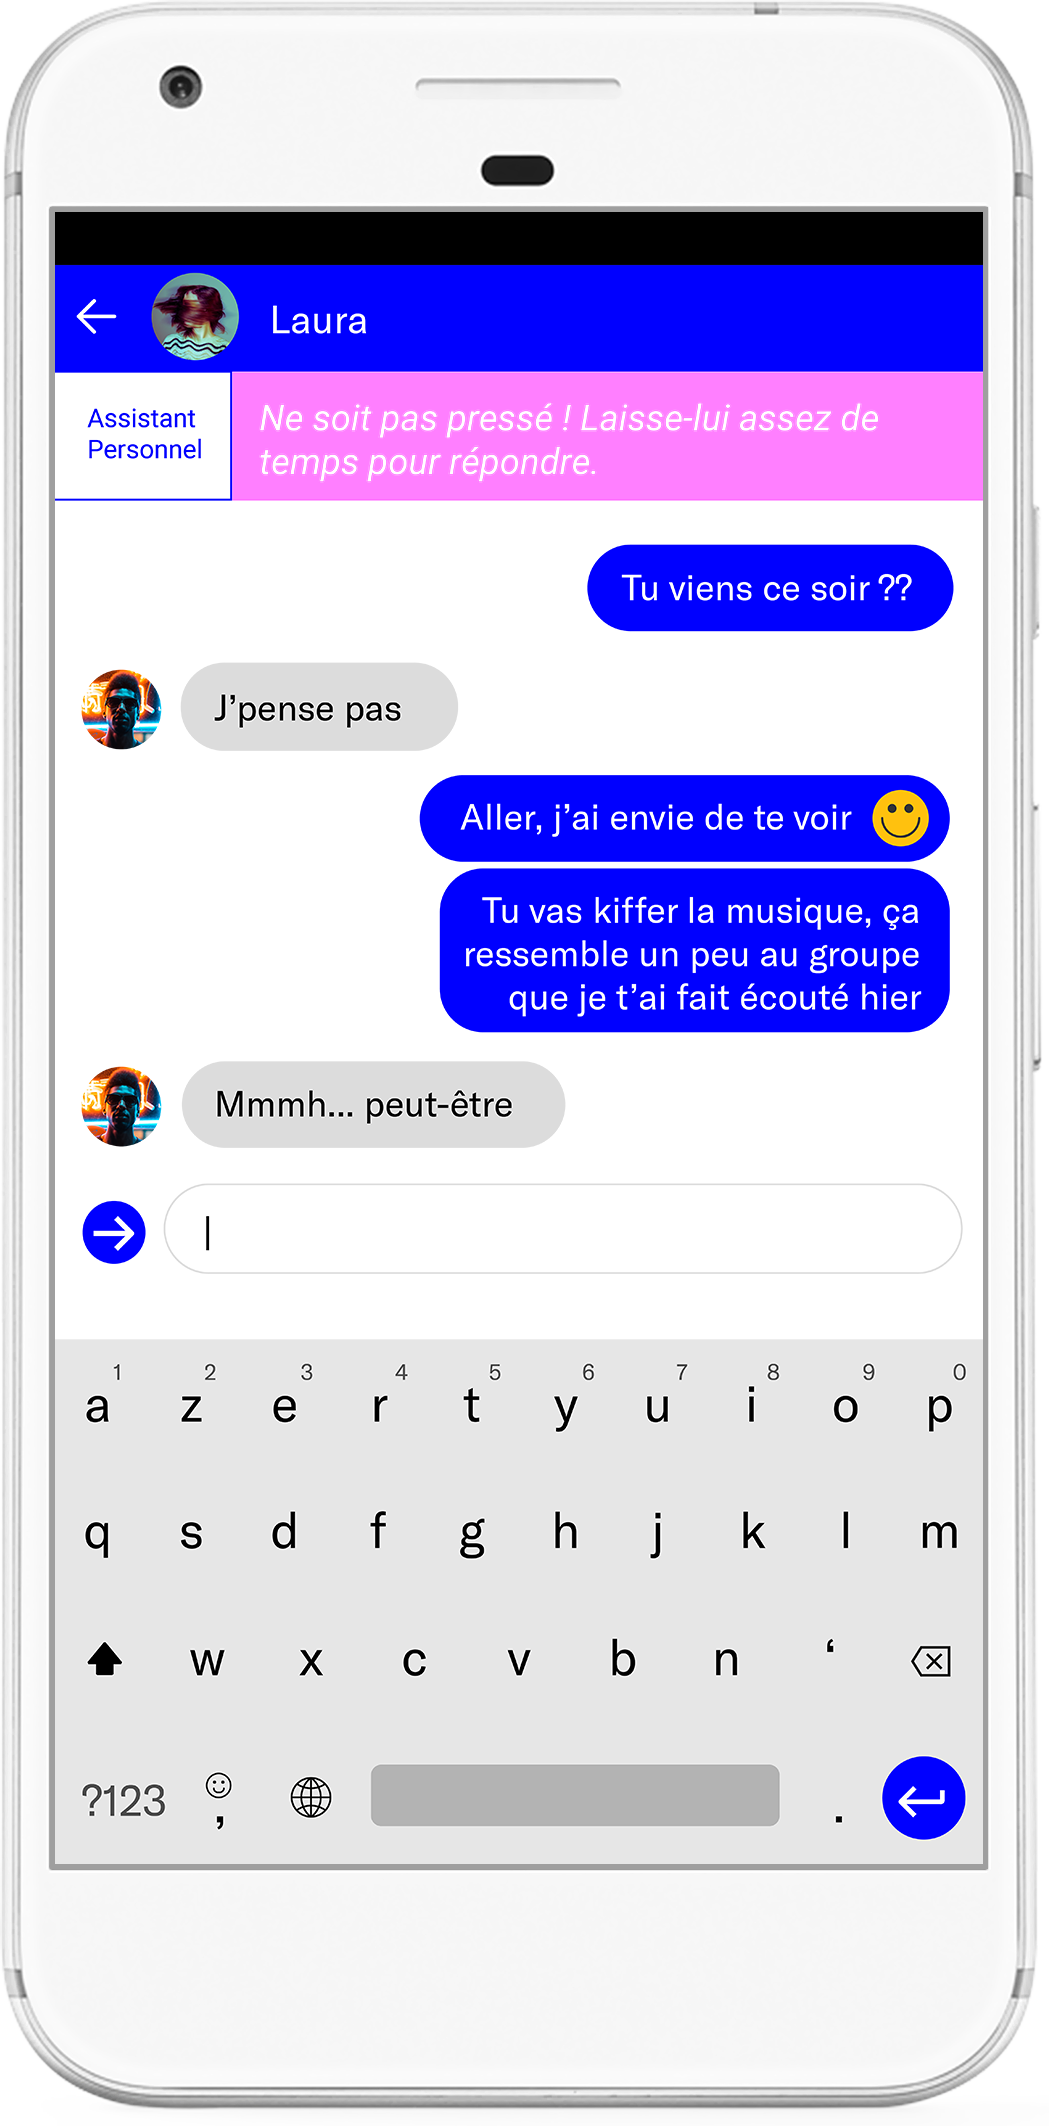
\includegraphics{./tex2pdf.9048/88954f3f29fc76e5680ebca2dcb65ebaed1db248.png}
\caption{Et si\ldots{} on pouvait recevoir en temps réel des conseils
pour améliorer sa manière de converser ?}
\end{figure}

\newpage

\hypertarget{templates-de-conversation}{%
\subsubsection{Templates de
conversation}\label{templates-de-conversation}}

\begin{figure}
\centering
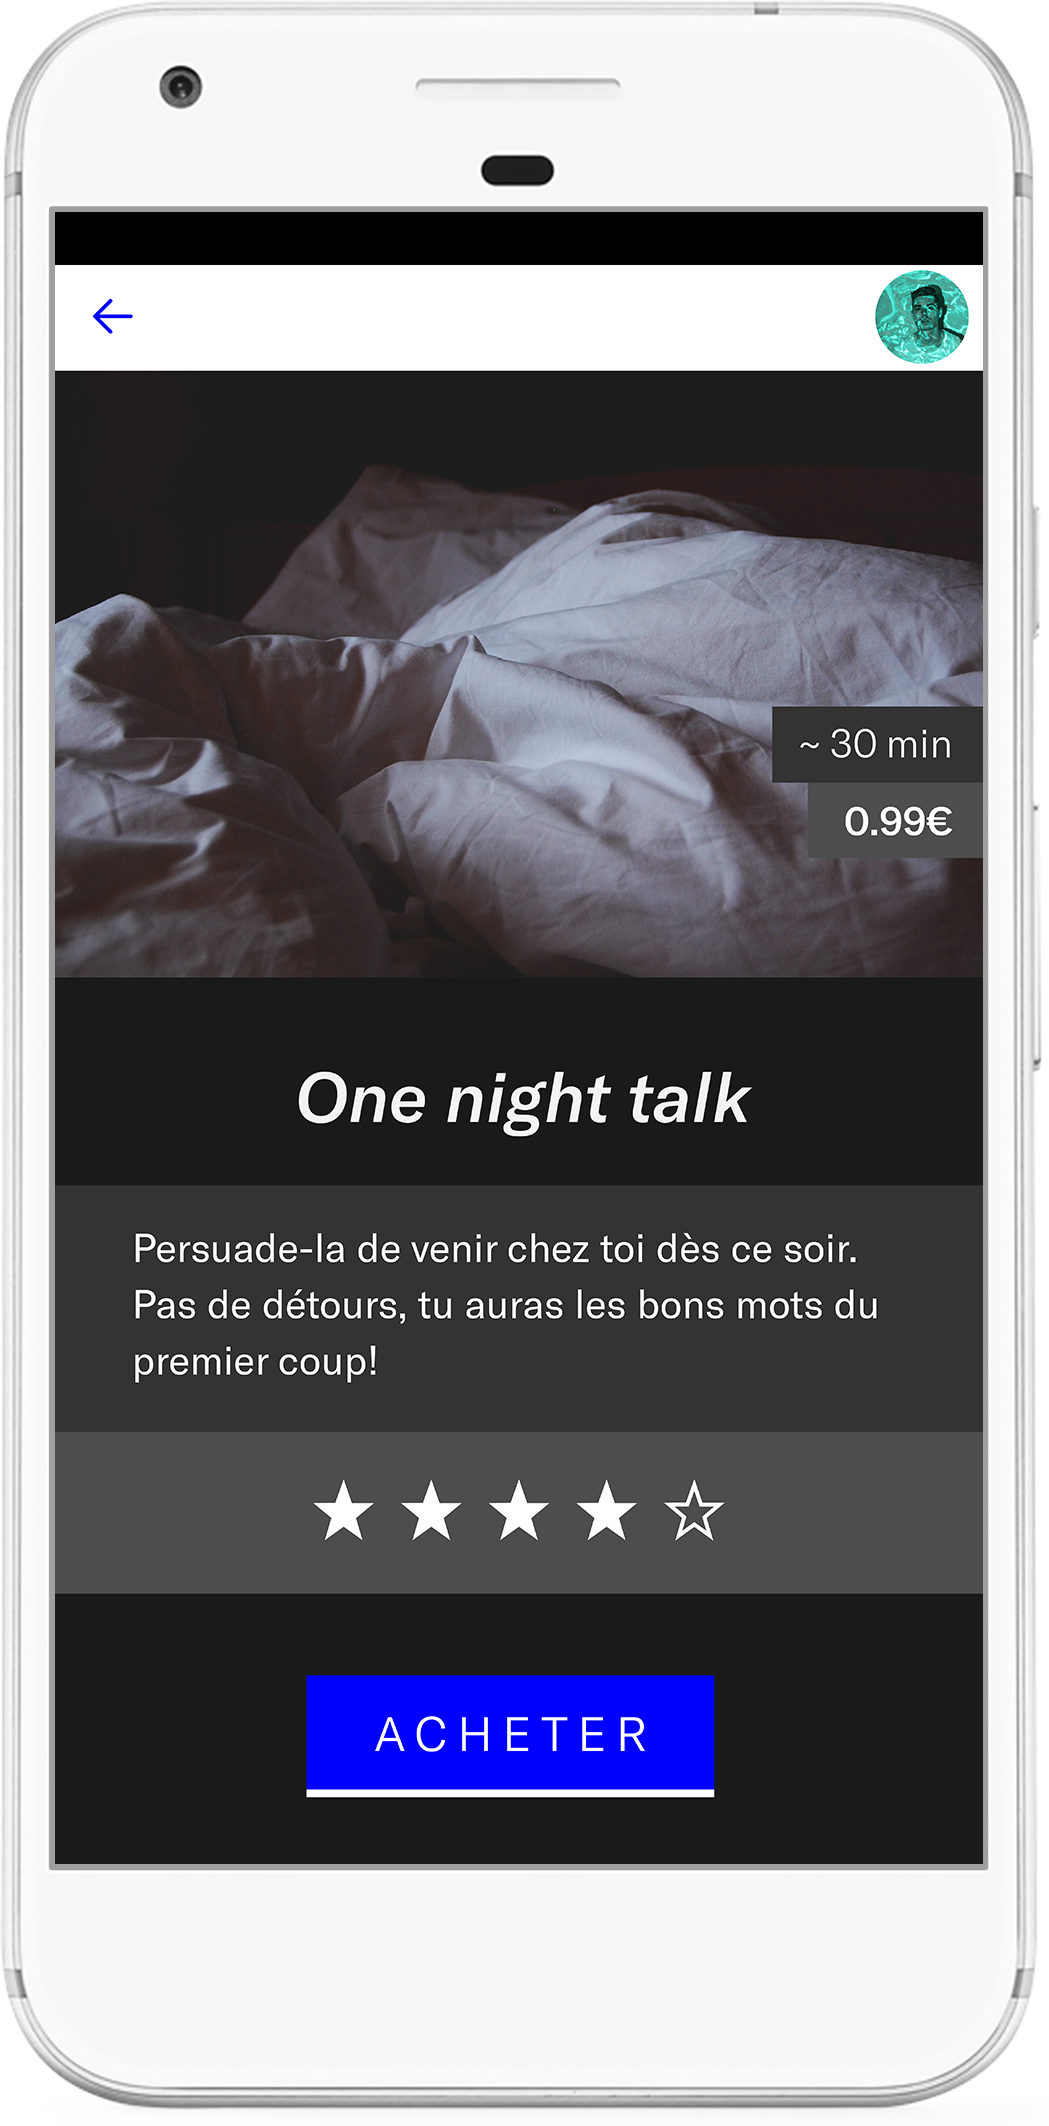
\includegraphics{./tex2pdf.9048/f32fb5cd3e27171f4e5bc0b3fcc0c23743d22cd0.png}
\caption{Et si\ldots{} on pouvait télécharger (ou acheter) des templates
de conversation ? Pour ne jamais être à court d'idées ?}
\end{figure}

\newpage

\hypertarget{ecrire-dans-le-style-de}{%
\subsubsection{Ecrire dans le style
de\ldots{}}\label{ecrire-dans-le-style-de}}

\begin{figure}
\centering
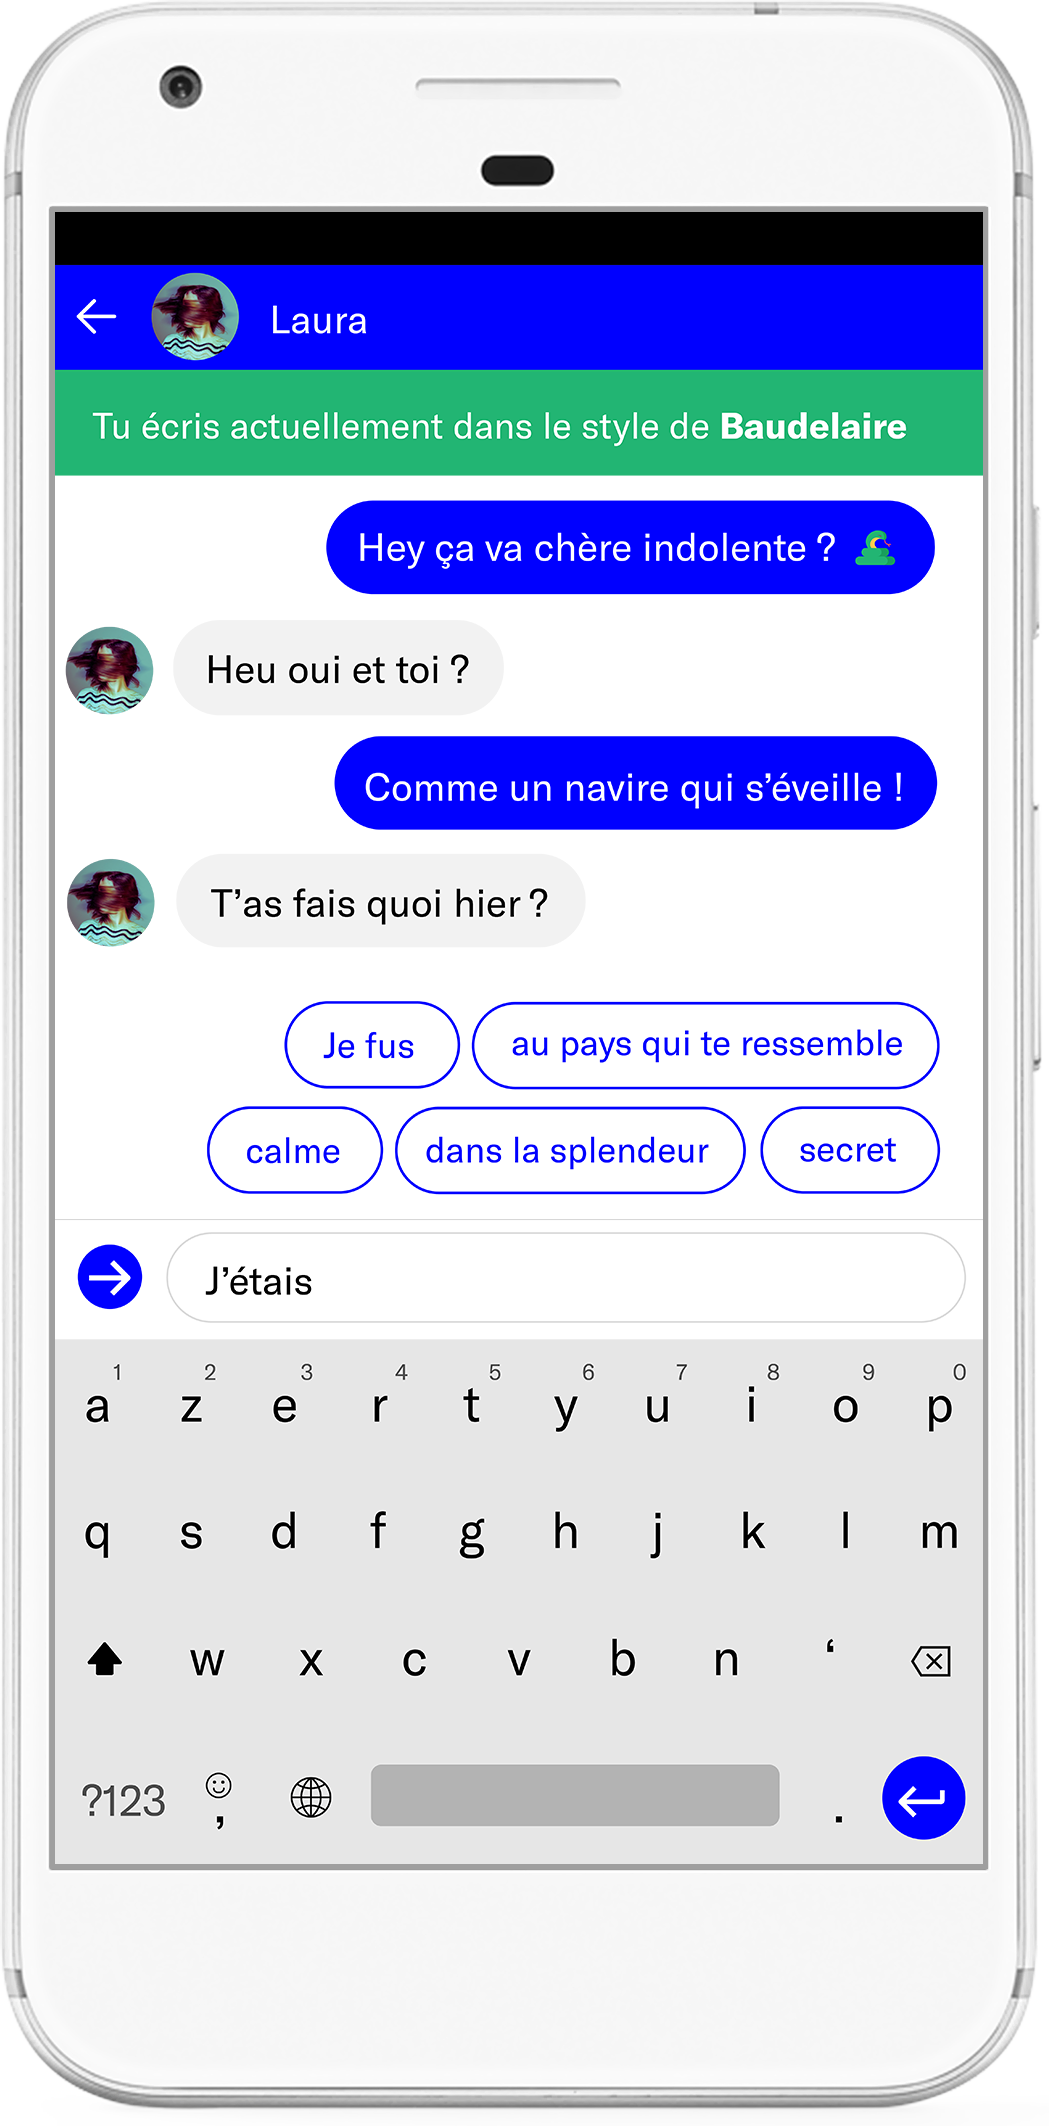
\includegraphics{./tex2pdf.9048/d8ebd9f7ed07cdf560a05a9e56096918a37071f0.png}
\caption{Et si\ldots{} on pouvait écrire dans le style des meilleurs
écrivains ?}
\end{figure}

\newpage

\hypertarget{gestionnaire-de-personnalituxe9}{%
\subsubsection{Gestionnaire de
personnalité}\label{gestionnaire-de-personnalituxe9}}

\begin{figure}
\centering
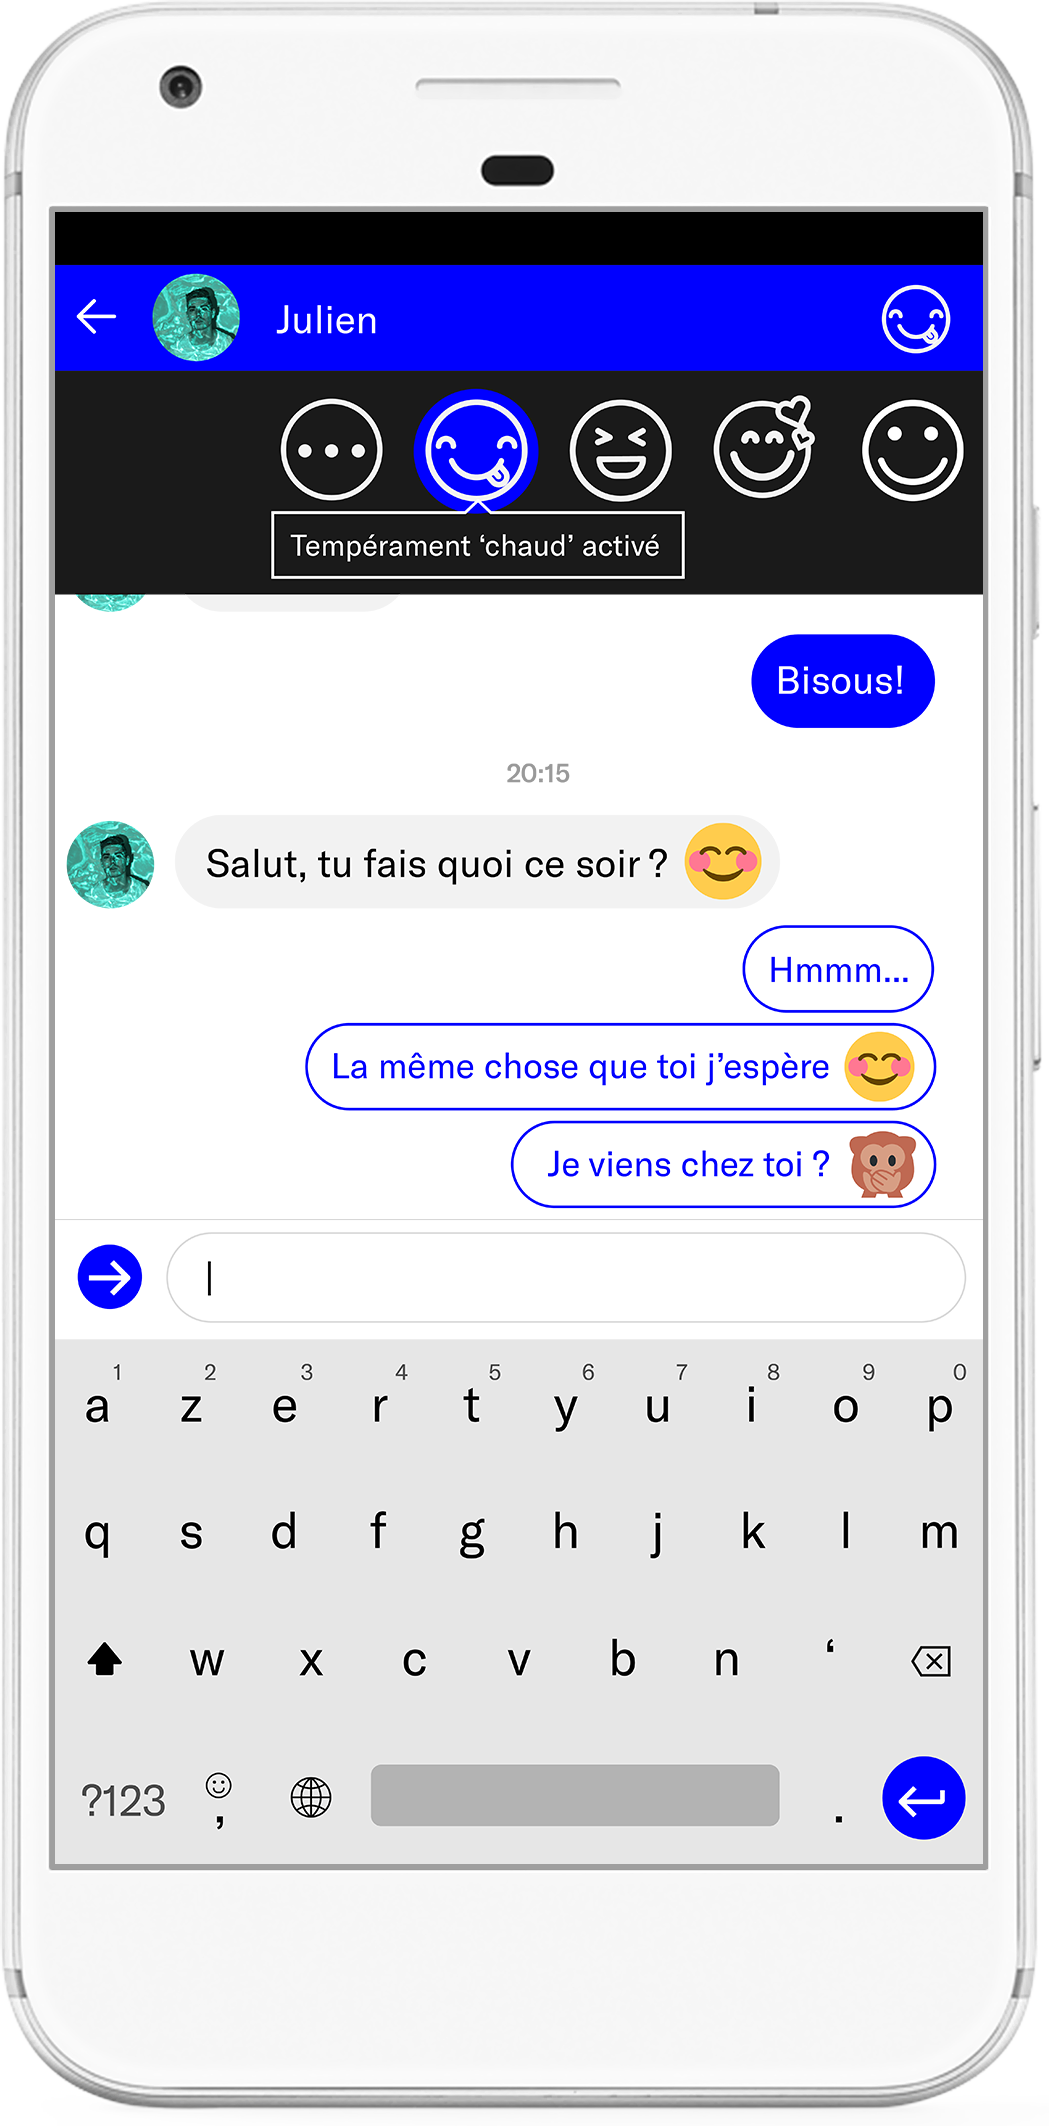
\includegraphics{./tex2pdf.9048/4e1335c1a8e7e8185fea4fb005bd843730ddc63c.png}
\caption{Et si\ldots{} on pouvait changer son tempéramment en fonction
du moment de la journée ou de la personne avec laquelle on parle, et
ainsi obtenir des recommandations compatibles avec notre humeur ?}
\end{figure}

\newpage

\hypertarget{gestionnaire-de-vocabulaire}{%
\subsubsection{Gestionnaire de
vocabulaire}\label{gestionnaire-de-vocabulaire}}

\begin{figure}
\centering
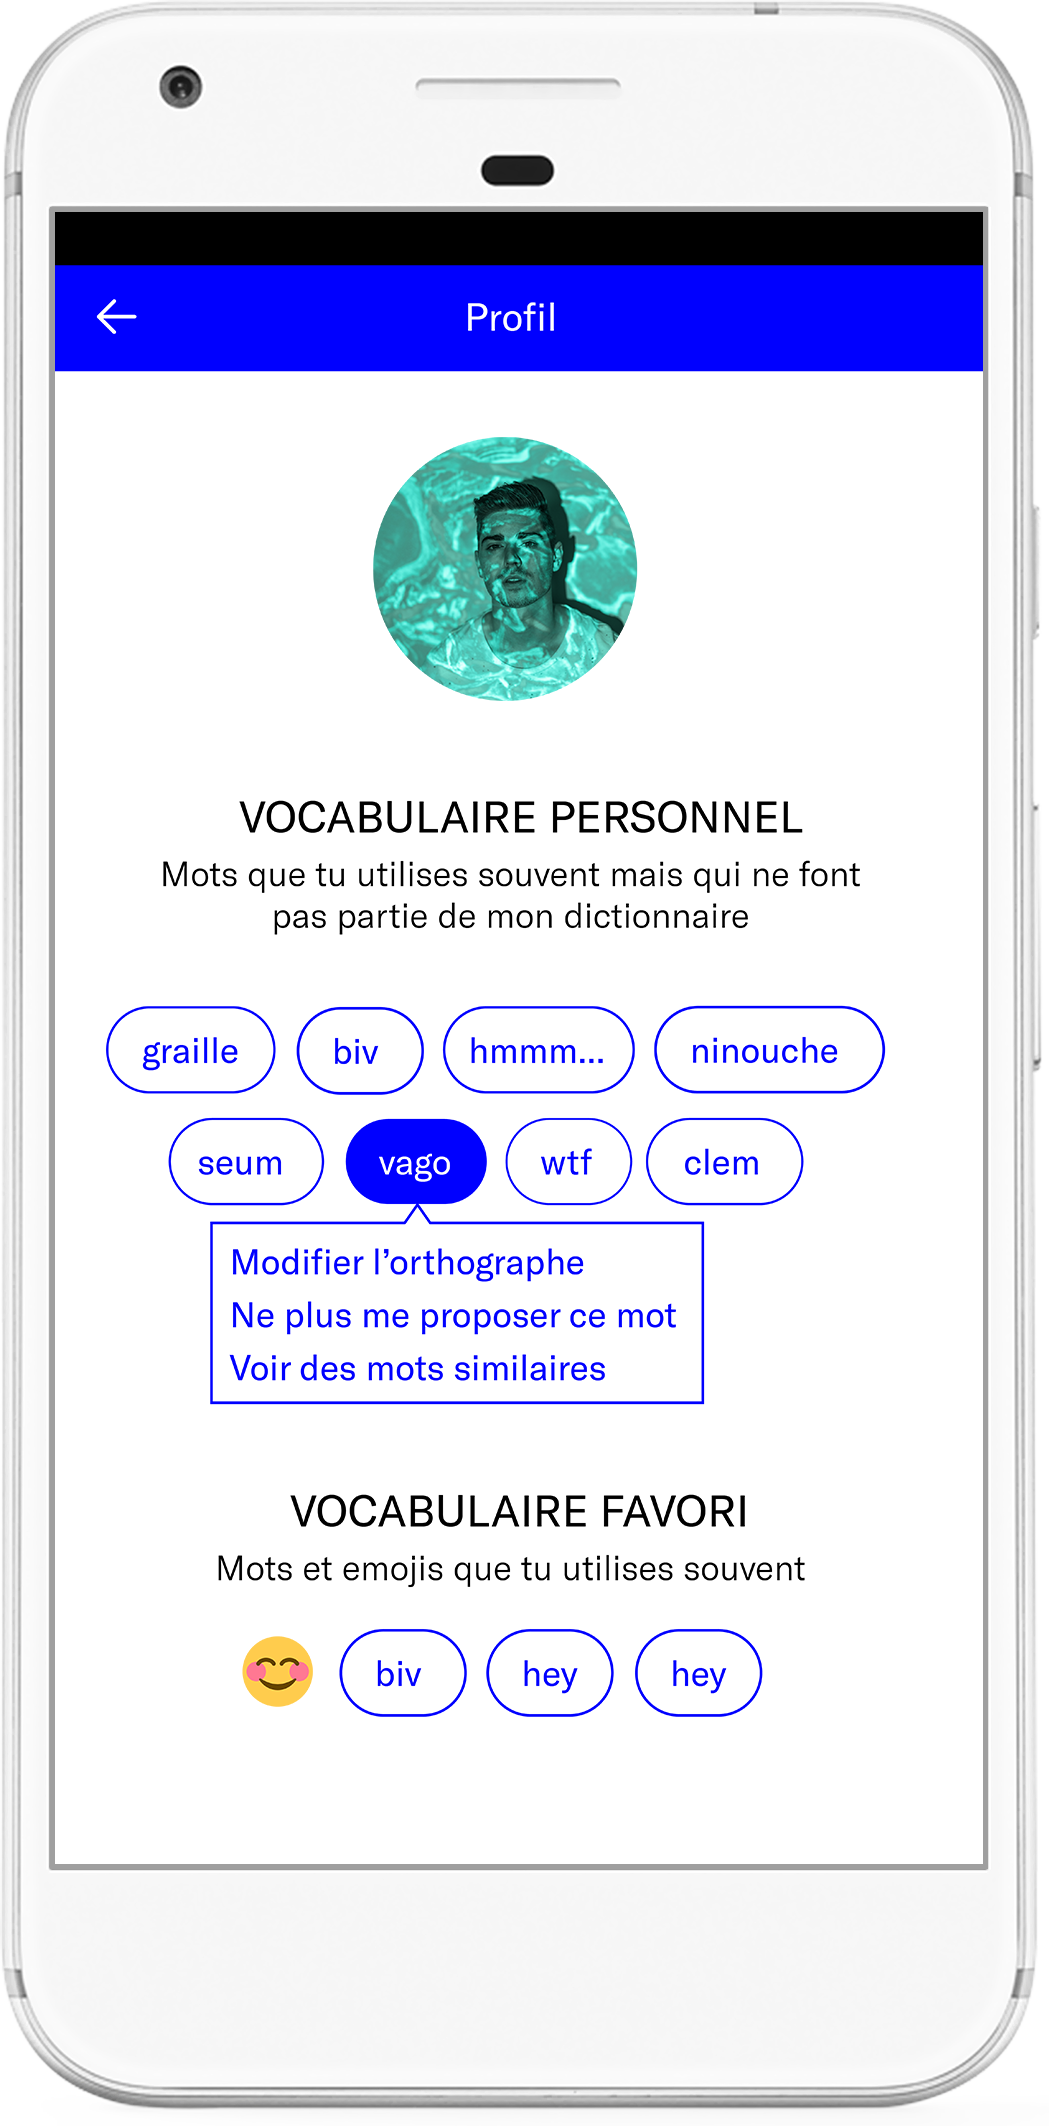
\includegraphics{./tex2pdf.9048/b1d1e37c73b5b566f821fe617c54dc9fb4f442b5.png}
\caption{Et si\ldots{} on pouvait contrôler précisemment son vocabulaire
: ajouter, modifier ou supprimer des mots ? Et même, apprendre des mots
nouveaux ?}
\end{figure}

\newpage

\hypertarget{diffuxe9rencier-les-mots-compluxe9tuxe9s}{%
\subsubsection{Différencier les mots
complétés}\label{diffuxe9rencier-les-mots-compluxe9tuxe9s}}

\begin{figure}
\centering
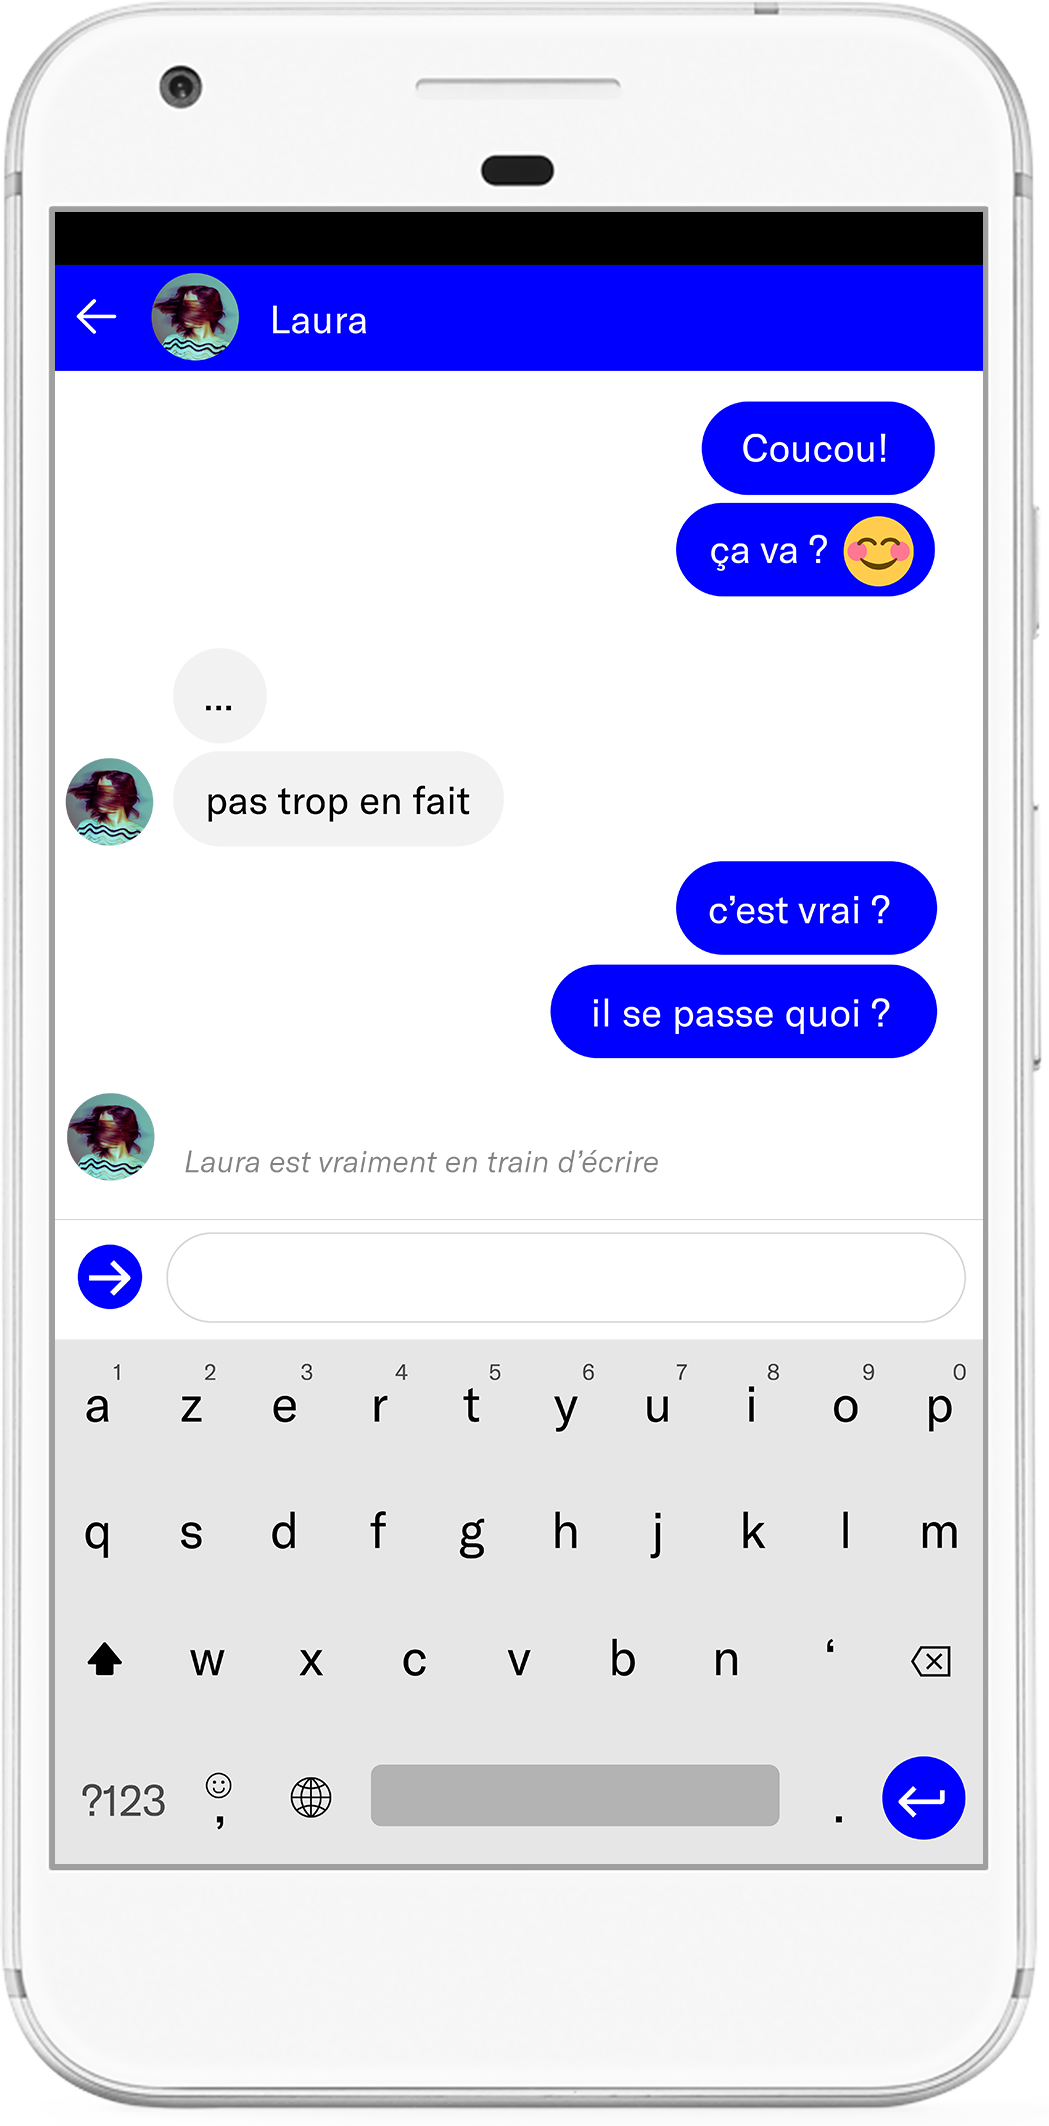
\includegraphics{./tex2pdf.9048/3cf5d895b47893617a467acf262ec2d2ab2cf793.png}
\caption{Et si\ldots{} l'autocomplétion devenait tellement utilisée
qu'il serait nécessaire de préciser quand quelqu'un écrit ``réellement''
?}
\end{figure}

\newpage

Imprimé à la HEAD - Genève, avec le caractères typographique GT America.

Ce texte est également disponible en ligne sur le site internet
alternative.mathildebuenerd.fr/memoire

\newpage

\hypertarget{bibliographie}{%
\subsection{Bibliographie}\label{bibliographie}}

\hypertarget{iconographie}{%
\subsubsection{Iconographie}\label{iconographie}}

\hypertarget{schuxe9ma-filtrage-collaboratif-filtrage-basuxe9-sur-le-contenu}{%
\paragraph{Schéma filtrage collaboratif / filtrage basé sur le
contenu}\label{schuxe9ma-filtrage-collaboratif-filtrage-basuxe9-sur-le-contenu}}

Schéma inspiré de : http://i65.tinypic.com/2ebah6c.png Emojis : Par
Twitter, www.flaticon.com Personnages : Par Freepik, www.flaticon.com

\hypertarget{annexe}{%
\paragraph{Annexe}\label{annexe}}

\begin{itemize}
\tightlist
\item
  Mock-up téléphone : designed by Vexels.com
\item
  Interfaces :

  \begin{itemize}
  \tightlist
  \item
    Design par Mathilde Buenerd
  \item
    Emojis par Twitter ou Freepik, www.flaticon.com
  \item
    Photographies par www.unsplash.com
  \end{itemize}
\end{itemize}

\hypertarget{refs}{}
\leavevmode\hypertarget{ref-zotero-89}{}%
``A Mobile Keyboard by Plan International Boosts Girls' Confidence.''
n.d. https://www.sheboard.com.

\leavevmode\hypertarget{ref-Arnall2013}{}%
Arnall, Timo. 2013. ``No to NoUI.'' \emph{Elastic Space}.

\leavevmode\hypertarget{ref-Barthes1953}{}%
Barthes, Roland. 1953. \emph{Le Degré zéro de l'écriture}. Le Seuil.

\leavevmode\hypertarget{ref-Bian2017}{}%
Bian, Lin, Sarah-Jane Leslie, and Andrei Cimpian. 2017. ``Gender
Stereotypes About Intellectual Ability Emerge Early and Influence
Children's Interests.'' \emph{Science} 355 (January):389--91.
\url{https://doi.org/10.1126/science.aah6524}.

\leavevmode\hypertarget{ref-Caruana2015}{}%
Caruana, Rich, Yin Lou, Johannes Gehrke, Paul Koch, Marc Sturm, and
Noemie Elhadad. 2015. ``Intelligible Models for HealthCare: Predicting
Pneumonia Risk and Hospital 30-Day Readmission.'' In \emph{Proceedings
of the 21th ACM SIGKDD International Conference on Knowledge Discovery
and Data Mining}, 1721--30. KDD '15. New York, NY, USA: ACM.
\url{https://doi.org/10.1145/2783258.2788613}.

\leavevmode\hypertarget{ref-Christie2017}{}%
Christie, Alex. 2017. ``Smooth Talk - Proofreading Apps Gloss over the
Meaning of Our Words.'' \emph{Real Life}.

\leavevmode\hypertarget{ref-Citton2015}{}%
Citton, Yves. 2015. ``Herméneutique et (re)médiation : vers des études
de media comparés ?'' \emph{Critique}, nos. 817-818 (June):569--81.

\leavevmode\hypertarget{ref-Feron}{}%
Feron, Christian. n.d. ``Le Criticon'Art, générateur de critiques d'art
contemporain en ligne.''
http://chrisferon.free.fr/technologies-langage/criticon-art.php.

\leavevmode\hypertarget{ref-Finn2017}{}%
Finn, Ed. 2017. \emph{What Algorithms Want : Imagination in the Age of
Computing}. Cambridge, Mass: The MIT Press.

\leavevmode\hypertarget{ref-Gillespieed.2014}{}%
Gillespie (ed.), Tarleton, Pablo J. Boczkowski (ed.), and Kirsten A.
Foot (ed.). 2014. \emph{Media Technologies: Essays on Communication,
Materiality, and Society}. 1st ed. Inside Technology. The MIT Press.

\leavevmode\hypertarget{ref-Girardin2016}{}%
Girardin, Fabien. 2016. ``Experience Design in the Machine Learning
Era.'' \emph{Medium}.

\leavevmode\hypertarget{ref-Grover1998}{}%
Grover, Dale L., Martin T. King, and Clifford A. Kushler. 1998. Reduced
keyboard disambiguating computer. US5818437 (A), issued October 1998.

\leavevmode\hypertarget{ref-Hall2017}{}%
Hall, David. 2017. ``NoUI and the Danger of Invisible Design.''
\emph{David Hall}.

\leavevmode\hypertarget{ref-Hayles2005}{}%
Hayles, N. Katherine. 2005. \emph{My Mother Was a Computer: Digital
Subjects and Literary Texts}. 1st ed. University Of Chicago Press.

\leavevmode\hypertarget{ref-Hendler2016}{}%
Hendler, James, and Alice M. Mulvehill (auth.). 2016. \emph{Social
Machines: The Coming Collision of Artificial Intelligence, Social
Networking, and Humanity}. 1st ed. Apress.

\leavevmode\hypertarget{ref-Jacobi2005}{}%
Jacobi, Daniel. 2005. ``Discourir de l'œuvre de l'art contemporain. Le
cas des Détails.'' \emph{Linx. Revue Des Linguistes de L'université
Paris X Nanterre}, no. 52 (June):17--30.
\url{https://doi.org/10.4000/linx.170}.

\leavevmode\hypertarget{ref-Kaplan2007}{}%
Kaplan, Frederic. 2007. ``Beyond Robotics.'' \emph{Vimeo}.
https://vimeo.com/6453775.

\leavevmode\hypertarget{ref-Kaplan2014}{}%
---------. 2014. ``Linguistic Capitalism and Algorithmic Mediation.''
\emph{Representations} 127 (1):57--63.
\url{https://doi.org/10.1525/rep.2014.127.1.57}.

\leavevmode\hypertarget{ref-Krishna2015}{}%
Krishna, Golden. 2015. \emph{The Best Interface Is No Interface: The
Simple Path to Brilliant Technology}. San Francisco, Calif.: New Riders.

\leavevmode\hypertarget{ref-zotero-28}{}%
``MACH - My Automated Conversation coacH.'' n.d.
http://hoques.com/MACH.htm.

\leavevmode\hypertarget{ref-Manny2017}{}%
Manny. 2017. ``The Business Case for Machine Learning
Interpretability.'' \emph{Fast Forward Labs}.

\leavevmode\hypertarget{ref-Masure2016}{}%
Masure, Anthony. 2016. ``Subjectivités computationnelles et consciences
appareillées.'' \emph{Multitudes}, no. 62 (April):87--96.
\url{https://doi.org/10.3917/mult.062.0087}.

\leavevmode\hypertarget{ref-Maurer}{}%
Maurer, Luna, Edo Paulus, Jonathan Puckey, and Roel Wouters. n.d.
``Conditional Design Manifesto.''
https://conditionaldesign.org/manifesto/.

\leavevmode\hypertarget{ref-McNeil2014}{}%
McNeil, Joanne. 2014. ``The Internet of Things Will Ruin Birthdays.''
\emph{Medium}.

\leavevmode\hypertarget{ref-McQuillan2017}{}%
McQuillan, Dan. 2017. ``Data Science as Machinic Neoplatonism.''
\emph{Philosophy \& Technology}, August, 1--20.
\url{https://doi.org/10.1007/s13347-017-0273-3}.

\leavevmode\hypertarget{ref-2015}{}%
``"Means Well" Technology and the Internet of Good Intentions.'' 2015.
\emph{Thingclash}.
http://www.thingclash.com/blog/2015/8/15/means-well-technology-and-the-network-of-good-intentions.

\leavevmode\hypertarget{ref-Pariser2011}{}%
Pariser, Eli. 2011. \emph{The Filter Bubble: What the Internet Is Hiding
from You}. Penguin Press HC, The.

\leavevmode\hypertarget{ref-Poole2008}{}%
Poole, Erika Shehan, Christopher A. Le Dantec, James R. Eagan, and W.
Keith Edwards. 2008. ``Reflecting on the Invisible: Understanding
End-User Perceptions of Ubiquitous Computing.'' In \emph{Proceedings of
the 10th International Conference on Ubiquitous Computing}, 192--201.
UbiComp '08. New York, NY, USA: ACM.
\url{https://doi.org/10.1145/1409635.1409662}.

\leavevmode\hypertarget{ref-Ratto2007}{}%
Ratto, Matt. 2007. ``Ethics of Seamless Infrastructures : Resources and
Future Directions.'' \emph{International Review of Information Ethics} 8
(8):20--27.

\leavevmode\hypertarget{ref-Sheret2017}{}%
Sheret, Matthew. 2017. ``Making It Clear When Machines Make Decisions.''
\emph{Projects by If Blog}.

\leavevmode\hypertarget{ref-Silfverberg2000}{}%
Silfverberg, Miika, I. Scott MacKenzie, and Panu Korhonen. 2000.
``Predicting Text Entry Speed on Mobile Phones.'' In \emph{Proceedings
of the SIGCHI Conference on Human Factors in Computing Systems}, 9--16.
CHI '00. New York, NY, USA: ACM.
\url{https://doi.org/10.1145/332040.332044}.

\leavevmode\hypertarget{ref-zotero-52}{}%
``The Original Hacker's Dictionary.'' n.d.
http://www.dourish.com/goodies/jargon.html.

\leavevmode\hypertarget{ref-Thornton2017}{}%
Thornton, Pip. 2017. ``Subprime Language: The Changing Value of Words in
an Age of Digital Linguistic Capitalism.'' \emph{RESEARCH VALUES 2018}.

\leavevmode\hypertarget{ref-Turing1950}{}%
Turing, A. M. 1950. ``Computing Machinery and Intelligence.''
\emph{Mind} 59 (236):433--60.

\leavevmode\hypertarget{ref-zotero-30}{}%
``US+.'' n.d. \emph{21st Century Digital Art}.
http://www.digiart21.org/art/us.

\leavevmode\hypertarget{ref-Weiser1995}{}%
Weiser, Mark, and John Seely Brown. 1995. ``Designing Calm Technology.''
http://www.ubiq.com/hypertext/weiser/calmtech/calmtech.htm.

\leavevmode\hypertarget{ref-Weizenbaum1981}{}%
Weizenbaum, Joseph. 1981. \emph{Puissance de l'ordinateur et raison de
l'homme: du jugement au calcul}. Ed. d'informatique.

\end{document}
